\documentclass[12pt,a4paper]{report}

%\includeonly{cover/cimlap, chapters/1_introduction}

\usepackage{styles/dolgozat}

% programkód beillesztéséhez
\usepackage{listings}
% listing float neve
\renewcommand{\lstlistingname}{Programkód}
%\renewcommand{\lstlistlistingname}{Programkódok listája}
% ékezetes betűk a kódrészletekben (pdfLaTeX + listings esetén kell)
\lstset{inputencoding=utf8,extendedchars=true,breaklines=true,literate=
  {á}{{\'a}}1 {é}{{\'e}}1 {í}{{\'i}}1 {ó}{{\'o}}1 {ö}{{\"o}}1 {ő}{{\H{o}}}1
  {ú}{{\'u}}1 {ü}{{\"u}}1 {ű}{{\H{u}}}1
  {Á}{{\'A}}1 {É}{{\'E}}1 {Í}{{\'I}}1 {Ó}{{\'O}}1 {Ö}{{\"O}}1 {Ő}{{\H{O}}}1
  {Ú}{{\'U}}1 {Ü}{{\"U}}1 {Ű}{{\H{U}}}1 {–}{{--}}1}
%saját listings style-ok, és a style-t használó parancsok definíciói
%\usepackage{styles/cpp}
\usepackage{styles/python}
\usepackage{styles/typescript}
%\usepackage{styles/java}
%\usepackage{styles/rust}

%% egyéb csomagok betöltése itt, vagy a dolgozat.sty fájlban
\usepackage{booktabs}
\usepackage{tabularx}
\usepackage{longtable}
% diagramok
\usepackage{tikz}
\usetikzlibrary{positioning,arrows.meta,shapes.multipart,fit,calc}
% jobb sorkizárás; a nem elválasztható (írógépbetűs) szavak ne lógjanak ki a margóra
\usepackage{microtype}
\setlength{\emergencystretch}{2em}
% URL-ek törése az irodalomjegyzékben bármely karakternél
\setcounter{biburlnumpenalty}{100}
\setcounter{biburllcpenalty}{100}
\setcounter{biburlucpenalty}{100}

% Kitöltendő helyek jelölése: pirosan látszik a PDF-ben, hogy ne maradjon benne
\newcommand{\todo}[1]{\textcolor{red}{\textbf{[#1]}}}

\usepackage{hyperref}
% cleveref csomag és beállításai -- az egyetlen, amit a hyperref után kell betölteni!
\usepackage{styles/refs}

\newcommand{\dolgozatCim}{Intelligens online vizsgáztató rendszer fejlesztése automatikus kódértékeléssel és valós idejű felügyelettel}
\newcommand{\hallgatoNev}{Kiss László}
\newcommand{\neptunKod}{EW9LOS}
\newcommand{\szak}{Programtervező informatikus}
\newcommand{\temavezetoNev}{Dr. Agárdi Anita}
\newcommand{\temavezetoBeosztas}{egyetemi adjunktus}
\newcommand{\tanszek}{Alkalmazott Matematikai Intézeti Tanszék}
\newcommand{\targykor}{webes alkalmazásfejlesztés, online vizsgáztatás, automatikus kódértékelés, konténerizáció, proctoring}
\newcommand{\ev}{2026}


\begin{document}

\pagestyle{empty}
\pagenumbering{gobble}

\begin{titlepage}
\centering
% A Miskolci Egyetem címere
\vspace*{2cm}
\huge\textsc{\textbf{Szakdolgozat}}\\[1cm]
%\vspace*{1cm}

\includegraphics[width=4.8cm, height=4cm,keepaspectratio]{images/me_logo.png}\\
\textbf{\textsc{Miskolci Egyetem}}

\vspace*{2cm}

% A szakdolgozat címe, akár több sorban is
{\LARGE\textbf{\dolgozatCim}\par}

\vspace*{2cm}
% A hallgató neve, évfolyam, szak(ok), a konzulens(ek) neve
\large
\textbf{Készítette:}\\[0.8ex]
\hallgatoNev\\[0.8ex]
\szak

\vspace*{0.5cm}
\textbf{Témavezető:}\\[0.8ex]
\temavezetoNev

\vfill

% Keltezés: Hely, év
\large
\textbf{\textsc{Miskolc, \ev}}

\end{titlepage}

%Feladatkiiras
\noindent
\textsc{\textbf{Miskolci Egyetem}}\\
Gépészmérnöki és Informatikai Kar\\
\tanszek\hspace*{4cm}\hfil \textbf{Szám:}

\vspace{0.5cm}
\begin{center}
\large\textsc{\textbf{Szakdolgozat Feladat}}
\end{center}
\vspace{0.5cm}

\hallgatoNev{} (\neptunKod) programtervező informatikus jelölt részére.

\bigskip
\noindent\textbf{A szakdolgozat tárgyköre:} \targykor

\bigskip
\noindent\textbf{A szakdolgozat címe:} \dolgozatCim

\bigskip
\noindent\textbf{A feladat részletezése:}

\medskip

% A HIVATALOS feladatkiírás szövegét kell ide szó szerint bemásolni!
A hallgató feladata egy webes online vizsgáztató rendszer prototípusának megtervezése és
megvalósítása, amely egy vizsgán belül többféle feladattípust kezel: egy- és több választós,
igaz--hamis, rövid szöveges, kifejtős és programozási feladatokat. A zárt végű feladatokat a
rendszer automatikusan pontozza, a kifejtős válaszokat az oktató kézzel értékelheti és szöveges
visszajelzéssel láthatja el. A programozási feladatok megoldásait a rendszer izolált
Docker-konténerben, korlátozott erőforrásokkal és hálózati hozzáférés nélkül futtatja, majd
nyilvános és rejtett tesztesetek alapján automatikusan értékeli. A vizsga időkorláttal,
automatikus mentéssel és lejáratkor automatikus beadással működjön, az oktató pedig valós időben
kapjon értesítést, ha egy hallgató a vizsga közben elhagyja a vizsgaablakot. A rendszer FastAPI
alapú backenddel, PostgreSQL adatbázissal és Next.js alapú frontenddel, szerepkör alapú
(oktató, hallgató) jogosultságkezeléssel készüljön, működését funkcionális és biztonsági
tesztekkel kell igazolni.

\vfill

\noindent\textbf{Témavezető:} \temavezetoNev{} (\temavezetoBeosztas)

% \noindent\textbf{Konzulens(ek):} (akkor kötelezõ, ha a témavezetõ nem valamelyik matematikai tanszékrõl való; de persze lehet egyébként is)\newline

\bigskip
\noindent\textbf{A feladat kiadásának ideje:}

%\noindent\textbf{A feladat beadásának határideje:}

\vspace{1.5cm}

\hfill\makebox[6cm]{\dotfill}

\hfill\makebox[6cm]{szakfelelős}

\clearpage

\vspace*{1cm}  
\begin{center}
\large\textsc{\textbf{Eredetiségi Nyilatkozat}}
\end{center}
\vspace*{2cm}  

Alulírott \textbf{\hallgatoNev}; Neptun-kód: \texttt{\neptunKod} a Miskolci Egyetem Gépészmérnöki és Informatikai Karának végzős Programtervező informatikus szakos hallgatója ezennel büntetőjogi és fegyelmi felelősségem tudatában nyilatkozom és aláírásommal igazolom, hogy \textit{\dolgozatCim}
című szakdolgozatom saját, önálló munkám; az abban hivatkozott szakirodalom
felhasználása a forráskezelés szabályai szerint történt.

\medskip
Tudomásul veszem, hogy szakdolgozat esetén plágiumnak számít:
\begin{itemize}
\item szószerinti idézet közlése idézőjel és hivatkozás megjelölése nélkül;
\item tartalmi idézet hivatkozás megjelölése nélkül;
\item más publikált gondolatainak saját gondolatként való feltüntetése.
\end{itemize}

Alulírott kijelentem, hogy a plágium fogalmát megismertem, és tudomásul veszem, hogy
plágium esetén szakdolgozatom visszautasításra kerül.

\vspace*{3cm}

\noindent Miskolc, \makebox[2cm]{\dotfill}. év \makebox[2cm]{\dotfill}. hó \makebox[2cm]{\dotfill}. nap

\vspace*{3cm}

\hfill\makebox[6cm]{\dotfill}

\hfill\makebox[6cm]{Hallgató}



\clearpage

\newcommand{\ki}{témavezető(k)}
\newsavebox{\alairas}
\begin{lrbox}{\alairas}
\begin{tabular}{c@{\hspace{2cm}}c}
\makebox[4cm]{\dotfill} & \makebox[5cm]{\dotfill} \\
dátum & \ki \\
\end{tabular}
\end{lrbox}
\newcommand{\dotline}{\makebox[5cm]{\dotfill}}
\newcommand{\shortdotline}{\makebox[3.5cm]{\dotfill}}

\noindent 1.
\begin{tabular}[t]{cl}
\multirow{2}{*}{A szakdolgozat feladat módosítása}
&szükséges (módosítás külön lapon) \\
& nem szükséges\\[1ex]
\end{tabular}

\begin{center}
\usebox{\alairas}
\end{center}

\smallskip

\noindent 2. A feladat kidolgozását ellenőriztem:

\begin{center}
\begin{tabular}{c@{\hspace*{2cm}}c}
témavezető (dátum, aláírás): & konzulens (dátum, aláírás):\\
\dotline & \dotline \\
\dotline & \dotline \\
\dotline & \dotline 
\end{tabular}
\end{center}

\smallskip

\noindent 3. A szakdolgozat beadható:

\begin{center}
\usebox{\alairas}
\end{center}

\noindent 4.
\begin{tabular}[t]{@{}l@{\hspace*{1mm}}l@{\hspace*{1mm}}l}
A szakdolgozat & \shortdotline & szövegoldalt\\
              & \shortdotline & program protokollt (listát, felhasználói leírást)\\
              & \shortdotline & elektronikus adathordozót (részletezve)\\
              & \shortdotline \\
              & \shortdotline & egyéb mellékletet (részletezve)\\
              & \shortdotline 
\end{tabular}
\newline tartalmaz.

\begin{center}
\usebox{\alairas}
\end{center}

\noindent 5.
\begin{tabular}[t]{ll}
\multirow{2}{*}{A szakdolgozat bírálatra} & bocsátható\\
& nem bocsátható\\
\end{tabular}

\smallskip

\noindent A bíráló neve: \makebox[8cm]{\dotfill}

\renewcommand{\ki}{szakfelelős}
\begin{center}
\begin{tabular}{c@{\hspace{2cm}}c}
\makebox[4cm]{\dotfill} & \makebox[5cm]{\dotfill} \\
dátum & \ki \\
\end{tabular}
\end{center}

\noindent 6.
\begin{tabular}[t]{lll}
A szakdolgozat osztályzata \\
& a témavezető javaslata: & \makebox[2.5cm]{\dotfill} \\
& a bíráló javaslata: & \makebox[2.5cm]{\dotfill} \\
& a szakdolgozat végleges eredménye: & \makebox[2.5cm]{\dotfill}
\end{tabular}

\bigskip\bigskip

\noindent Miskolc, \makebox[4cm]{\dotfill} \hfill \makebox[8cm]{\dotfill} 

\hfill \makebox[8cm]{a Záróvizsga Bizottság Elnöke} 


\tableofcontents

\clearpage
\pagenumbering{arabic}
\pagestyle{fancy}

%!TEX root = ../dolgozat.tex
\chapter{Bevezetés}
\label{ch:bevezetes}

A felsőoktatásban az elmúlt években alapvetően megváltozott a számonkérés módja. A
COVID-19 járvány idején az egyetemek kényszerből tértek át az online oktatásra és vizsgáztatásra,
a járvány elmúltával azonban sok intézmény megtartotta a digitális számonkérés bevált elemeit. Az
online vizsga gyorsabb értékelést, egységesebb pontozást és rugalmasabb szervezést tesz lehetővé, a
nagy létszámú évfolyamok oktatói számára pedig jelentős tehermentesítést jelent. Ugyanakkor
olyan kérdéseket is felvet, amelyekre a hagyományos, papíralapú vizsgáknál nem kellett választ
keresni: hogyan lehet megbízhatóan, igazságosan és biztonságosan értékelni a hallgatók munkáját,
és hogyan lehet meggyőződni arról, hogy a vizsgázó valóban önállóan dolgozott.

Különösen igaz ez az informatikai képzésekre. Egy programozási feladat megoldását nem elég
,,elolvasni'', a programot le is kell futtatni, és meg kell vizsgálni, hogy különböző bemenetekre
helyes eredményt ad-e. Ha ezt az oktató kézzel végzi, a javítás rendkívül időigényes, és a
pontozás könnyen következetlenné válik: ugyanazt a hibát az egyik dolgozatban észreveszi, a
másikban nem. Kézenfekvő megoldásnak tűnik a programok automatikus, tesztesetekkel történő
ellenőrzése, ez azonban újabb nehézséget hoz magával. A szervernek ilyenkor egy ismeretlen
személy által írt, tetszőleges programkódot kell futtatnia, amely hibából vagy szándékosan
megpróbálhat kárt tenni a rendszerben: végtelen ciklusba kerülhet, elfogyaszthatja a memóriát,
vagy hozzáférhet olyan adatokhoz, amelyekhez nem volna szabad.

Témaválasztásomat elsősorban saját hallgatói tapasztalataim motiválták. A tanulmányaim során
több online vizsgáztató rendszert is használtam, és azt tapasztaltam, hogy ezek vagy általános
célú tesztrendszerek, amelyek a programozási feladatok értékelésére nem alkalmasak, vagy
kifejezetten programozási versenyekre készült megoldások, amelyekből hiányoznak az egyetemi
vizsga megszokott elemei, például a vegyes feladattípusok és a kézi javítás lehetősége. Érdekelt,
hogy egy modern webes technológiákra épülő, átlátható felépítésű rendszerben hogyan lehet ezt a
kettőt összekapcsolni, és hogyan lehet a nem megbízható kód futtatását a gyakorlatban is
biztonságossá tenni.

Dolgozatom célja egy olyan webes vizsgáztató rendszer prototípusának megtervezése és
elkészítése, amely egy vizsgán belül különböző típusú feladatokat kezel (egy- és több
választós, igaz--hamis, rövid szöveges, kifejtős és programozási feladatokat), a programozási
feladatokat izolált Docker-konténerben, nyilvános és rejtett tesztesetekkel automatikusan
értékeli, és valós időben értesíti az oktatót, ha egy hallgató a vizsga közben elhagyja a
vizsgaablakot. A munka során a következő kérdésekre kerestem a választ: Milyen eszközökkel
futtatható biztonságosan egy nem megbízható forrásból származó program? Milyen pontozási
szabályok igazságosak a részben helyes válaszok esetén? Mennyit ér, és hol vannak a határai a
böngészőben megvalósítható vizsgafelügyeletnek?

A dolgozat felépítése a következő. \Aref{ch:koncepcio}. fejezetben a számítógéppel támogatott
értékelés, a programozási feladatok automatikus értékelése és az online vizsgafelügyelet
szakirodalmát tekintem át, bemutatom a hasonló célú rendszereket és a felhasznált
technológiákat, majd megfogalmazom a rendszerrel szemben támasztott követelményeket.
\Aref{ch:tervezes}. fejezet a rendszer architektúráját, adatmodelljét és a főbb folyamatok
tervét ismerteti. \Aref{ch:megvalositas}. fejezetben a megvalósítás érdekesebb részleteit
mutatom be, különös tekintettel a kódfuttatás biztonságára és a valós idejű felügyeletre.
\Aref{ch:teszteles}. fejezet a rendszer funkcionális és biztonsági tesztelésének eredményeit
tartalmazza, végül \aref{ch:osszefoglalas}. fejezetben összegzem az elért eredményeket, és
kitérek a továbbfejlesztési lehetőségekre.

%!TEX root = ../dolgozat.tex
\chapter{Koncepció}
\label{ch:koncepcio}

Ebben a fejezetben azt a szakmai hátteret mutatom be, amelyre a dolgozatban elkészített rendszer
épül. Először a számítógéppel támogatott értékelés általános kérdéseit és a különböző
feladattípusok automatikus pontozását tekintem át, majd részletesebben foglalkozom a programozási
feladatok automatikus értékelésével és a nem megbízható programkód biztonságos futtatásával.
Ezt követően az online vizsgafelügyelet módszereit és az ezekkel kapcsolatos etikai kérdéseket
vizsgálom, majd összehasonlítom a hasonló célú, már létező rendszereket. A fejezet végén
bemutatom a felhasznált technológiákat, és megfogalmazom a rendszerrel szemben támasztott
követelményeket.

\section{Számítógéppel támogatott értékelés}
\label{sec:caa}

A számítógéppel támogatott értékelés (\textit{computer-assisted assessment}, CAA) Bull és
McKenna meghatározása szerint minden olyan értékelési forma, amelyben a számítógép szerepet
játszik a feladatok kiosztásában, a válaszok összegyűjtésében, a pontozásban vagy az
eredmények elemzésében \cite{bull2004blueprint}. A fogalom tehát tágabb, mint az ,,online teszt'':
ide tartozik az is, ha a hallgató papíron dolgozik, de a válaszlapokat gép dolgozza fel, és az is,
ha a hallgató számítógépen ad be egy dolgozatot, amelyet azután az oktató kézzel értékel.
Dolgozatomban a fogalom szűkebb értelmében, a teljes egészében számítógépen zajló vizsgára
használom.

Az értékelés céljuk szerint két nagy csoportba sorolható. A \textit{formatív} értékelés a
tanulási folyamat közben ad visszajelzést a hallgatónak és az oktatónak arról, hol tart a
hallgató, és min kell még dolgoznia; ilyenek a gyakorló feladatok és az önellenőrző tesztek. A
\textit{szummatív} értékelés ezzel szemben egy tanulási szakasz végén méri a tudást, és
jellemzően érdemjegyben vagy pontszámban ölt testet; ilyen a félévközi zárthelyi dolgozat és a
vizsga \cite{bull2004blueprint}. A két forma eltérő követelményeket támaszt egy informatikai
rendszerrel szemben. Formatív értékelésnél a gyors és részletes visszajelzés a legfontosabb, a
csalás elleni védelem kevésbé lényeges, hiszen a hallgatónak magának sem érdeke, hogy
,,becsapja'' a gyakorló feladatot. Szummatív értékelésnél viszont a megbízhatóság, a
megismételhetőség és a vizsga tisztaságának biztosítása kerül előtérbe. Az általam készített
rendszer elsősorban szummatív értékelésre, vagyis vizsgáztatásra készült, de a kódfeladatok
próbafuttatási lehetősége és a nyilvános példatesztek formatív elemeket is visznek bele.

A számítógéppel támogatott értékelés előnyei közül a szakirodalom leggyakrabban a gyorsaságot, a
következetességet és a nagy létszámú csoportok kezelhetőségét emeli ki \cite{bull2004blueprint}.
Egy automatikusan pontozott feladatsor eredménye a beadás pillanatában rendelkezésre áll, és a
pontozás minden hallgatónál ugyanazon szabályok szerint történik, függetlenül attól, hogy az
oktató az első vagy a századik dolgozatot javítja. Az eredmények gépi formában állnak elő, így
könnyen elemezhetők: kiderül, mely feladatok bizonyultak túl könnyűnek vagy túl nehéznek, és
melyik témakörben teljesített gyengén az évfolyam. A hátrányok között leggyakrabban azt
említik, hogy az automatikusan értékelhető feladatok -- különösen a feleletválasztós kérdések --
elsősorban a tényszerű tudást mérik, a magasabb rendű gondolkodási készségek (elemzés,
értékelés, alkotás) mérésére kevésbé alkalmasak, a jó minőségű feladatok összeállítása pedig
jelentős előkészítő munkát igényel \cite{bull2004blueprint}. Saját véleményem szerint ez a
probléma az informatikai képzésben részben feloldható: egy programozási feladat megoldása maga
is alkotó tevékenység, amely ráadásul jól automatizálható módon ellenőrizhető.

\section{Feladattípusok és automatikus pontozásuk}
\label{sec:feladattipusok}

A vizsgafeladatok a válasz kötöttsége szerint zárt, félig nyílt és nyílt feladatokra oszthatók. A
zárt feladatoknál a hallgató előre megadott lehetőségek közül választ; ide tartoznak az
egyválasztós, a több választós és az igaz--hamis kérdések. Ezek pontozása egyértelmű és teljes
mértékben automatizálható, hiszen csak azt kell megvizsgálni, hogy a megjelölt válaszok
egyeznek-e a megoldókulccsal. A félig nyílt feladatoknál a hallgató maga írja be a választ, de
annak formája kötött: egy szám, egy kifejezés vagy egy rövid szöveg. Ezek automatikus értékelése
már nem triviális, hiszen ugyanaz a helyes válasz többféleképpen is leírható (kis- vagy
nagybetűvel, szóközökkel, tizedesvesszővel vagy -ponttal), ezért az összehasonlítás előtt a
válaszokat egységes formára kell hozni, és célszerű több elfogadott választ is megengedni. A
nyílt feladatok, például a kifejtős kérdések, a mai eszközökkel megbízhatóan nem értékelhetők
automatikusan, ezeknél a számítógép szerepe a válaszok összegyűjtésére és a kézi javítás
támogatására korlátozódik.

Külön figyelmet érdemel a több helyes választ tartalmazó feladatok pontozása. Ha a rendszer csak a
tökéletes választ fogadja el, akkor egyetlen elnézett jelölés is nulla pontot eredményez, ami a
hallgató tudását nem tükrözi hűen. Ha viszont minden helyes jelölésért részpont jár, és a hibás
jelölésekért nem jár levonás, akkor a hallgató egyszerűen az összes lehetőséget megjelölheti, és
így biztosan megkapja a teljes pontszámot. A gyakorlatban ezért elterjedt megoldás, hogy a helyes
jelölések részpontot érnek, a hibás jelölések pedig ugyanilyen mértékben csökkentik a pontszámot,
de a feladatra adott pontszám nem lehet negatív. A rendszeremben ezt a pontozási módot
valósítottam meg (lásd \aref{sec:pontozas}. szakaszt), mert véleményem szerint ez egyensúlyt teremt
a részleges tudás elismerése és a találgatás visszaszorítása között.

\section{Programozási feladatok automatikus értékelése}
\label{sec:apas}

A programozási feladatok automatikus értékelése egyidős a programozásoktatással. Már 1960-ban
megjelent egy cikk, amely egy olyan programról számolt be, amely a hallgatók által lyukkártyán
beadott programokat futtatta le és értékelte \cite{hollingsworth1960automatic}. Douce és szerzőtársai
áttekintő tanulmányukban a terület fejlődését három generációra osztották
\cite{douce2005automatic}. Az első generáció rendszerei egy-egy konkrét környezethez kötött,
egyedi megoldások voltak. A második generáció általánosabb, parancssori és grafikus
eszközöket hozott, amelyek már több feladattípust és programozási nyelvet támogattak. A harmadik
generációt a webes rendszerek jelentik, amelyekben a hallgató böngészőből adja be a megoldását, és
az eredményt is ott kapja meg.

Ihantola és szerzőtársai a 2006 és 2010 között megjelent rendszereket vizsgálva arra a
következtetésre jutottak, hogy bár sok rendszer készült, ezek jelentős része egy-egy intézmény
belső eszköze maradt, és a rendszerek közötti legfontosabb különbségek a támogatott programozási
nyelvekben, a tesztek megadásának módjában, az újrabeküldés szabályaiban, a kézi értékelés
lehetőségében és a futtatás biztonságában mutatkoznak meg \cite{ihantola2010review}. Különösen az
utolsó szempontot emelték ki: egy automatikus értékelő rendszernek úgy kell futtatnia a
hallgatók programjait, hogy azok ne veszélyeztethessék sem a szervert, sem más hallgatók
megoldásait. Paiva és szerzőtársai egy jóval újabb, 2022-es áttekintésükben megállapították, hogy
az automatikus értékelés mára a számítástechnika-oktatás széles körben használt eszközévé vált,
és a kutatások súlypontja egyre inkább a hallgatónak adott visszajelzés minőségére helyeződik át
\cite{paiva2022automated}.

Az értékelés módszerei alapvetően két csoportba sorolhatók \cite{paiva2022automated}. A
\textit{dinamikus} elemzés a programot ténylegesen lefuttatja, és a viselkedését vizsgálja;
ennek legelterjedtebb formája a tesztelésen alapuló értékelés, amelyben a program előre megadott
bemenetekre adott kimenetét hasonlítjuk össze az elvárt kimenettel. A \textit{statikus} elemzés
a programot futtatás nélkül, a forráskód alapján vizsgálja, például a kódolási stílus, a
bonyolultság vagy bizonyos tiltott nyelvi elemek használata szempontjából. Rendszeremben a
dinamikus, tesztelésen alapuló értékelést valósítottam meg, mert ez közvetlenül azt méri, amit a
vizsgafeladat számon kér: hogy a program helyesen oldja-e meg a feladatot.

A tesztelésen alapuló értékelés egyik fontos tervezési kérdése, hogy a hallgató mennyit lásson a
tesztesetekből. Ha minden tesztesetet ismer, akkor fennáll a veszély, hogy a programját a konkrét
tesztekre ,,szabja'', például az elvárt kimeneteket egyszerűen kiírja, ahelyett hogy általános
megoldást készítene. Ha viszont egyet sem ismer, akkor nem tudja ellenőrizni, hogy jól értette-e
a feladatot, és például a kimenet formátumán (egy fölösleges szóközön vagy sortörésen) is
elbukhat. A gyakorlatban elterjedt kompromisszum a tesztesetek két csoportra bontása: a
nyilvános példatesztek a feladat megértését segítik, a rejtett tesztek pedig a megoldás
általánosságát ellenőrzik. Ezt a megoldást alkalmaztam a rendszeremben is.

\section{Nem megbízható programkód biztonságos futtatása}
\label{sec:sandbox_elmelet}

Az automatikus értékelő rendszer a hallgatók programjait futtatja, vagyis olyan kódot, amelynek
tartalmáról a futtatás előtt semmit sem tudunk. Egy ilyen programot -- a hibás és a szándékosan
ártó programokat egyaránt -- \textit{nem megbízható kódnak} nevezünk. A lehetséges fenyegetések
közé tartozik az erőforrások kimerítése (végtelen ciklus, korlátlan memóriafoglalás, rengeteg
folyamat indítása, óriási mennyiségű kimenet előállítása), a szerver fájljainak olvasása vagy
módosítása (például más hallgatók megoldásainak vagy a tesztesetek elvárt kimeneteinek
megszerzése), hálózati kapcsolatok kezdeményezése, valamint az értékelés eredményének
meghamisítása. A futtatókörnyezetet ezért úgy kell kialakítani, hogy a program csak a
számára kijelölt, szigorúan korlátozott erőforrásokhoz férhessen hozzá. Az ilyen elszigetelt
futtatókörnyezetet nevezzük homokozónak (\textit{sandbox}).

Az elszigetelésre több megoldás is létezik. A legegyszerűbb az operációs rendszer
folyamatszintű korlátozásainak használata (időkorlát, memóriakorlát, jogosultságok nélküli
felhasználó), ez azonban önmagában nem akadályozza meg, hogy a program lássa a szerver
fájlrendszerét és hálózatát. A másik véglet a teljes virtuális gép, amely erős elszigetelést nyújt,
de az indítása lassú és sok erőforrást igényel, ami egy vizsga során egyszerre beküldött több
száz megoldás esetén komoly korlátot jelent. A kettő között helyezkednek el a konténerek.

A Docker konténerek a Linux kernel két szolgáltatására épülnek \cite{merkel2014docker}. A
\textit{névterek} (\textit{namespaces}) segítségével a konténerben futó folyamat saját, elkülönített
nézetet kap a rendszerről: saját folyamatlistát, fájlrendszert, hálózati csatolókat és
felhasználókat lát, így a gazdagép többi folyamatához és fájljához nem fér hozzá. A
\textit{vezérlőcsoportok} (\textit{control groups}, cgroups) pedig lehetővé teszik a konténer által
felhasználható erőforrások -- memória, processzoridő, folyamatok száma -- korlátozását
\cite{docker_docs}. A konténer nem tartalmaz saját operációsrendszer-kernelt, hanem a gazdagépét
használja, ezért a virtuális gépeknél lényegesen gyorsabban, jellemzően egy másodpercen belül
elindul \cite{merkel2014docker}. Ennek az ára, hogy az elszigetelés gyengébb: egy kernelszintű
biztonsági rés esetén a konténerből elvileg ki lehet törni. Ezért a konténer jogosultságait is a
lehető legszűkebbre kell szabni: le kell tiltani a hálózatot, csak olvashatóvá kell tenni a
fájlrendszert, el kell dobni a Linux különleges jogosultságait (\textit{capabilities}), és a
programot nem rendszergazdaként kell futtatni. Az általam alkalmazott beállításokat \aref{tab:sandbox}.
táblázat foglalja össze.

\section{Online vizsgafelügyelet és akadémiai integritás}
\label{sec:proctoring}

Az online vizsgák egyik legtöbbet vitatott kérdése a vizsgázók felügyelete
(\textit{proctoring}). A felügyeleti megoldások három fő típusa különböztethető meg
\cite{nigam2021systematic}. Az \textit{élő felügyelet} során egy emberi felügyelő webkamerán
keresztül valós időben figyeli a vizsgázókat. A \textit{rögzített felügyelet} esetén a vizsga
alatt kép- és hangfelvétel készül, amelyet később egy felügyelő átnéz. Az \textit{automatizált
felügyelet} pedig mesterséges intelligenciára épülő módszerekkel elemzi a vizsgázó viselkedését,
és csak a gyanús eseteket jelzi emberi ellenőrzésre. Nigam és szerzőtársai rendszerező
áttekintésükben azt találták, hogy a COVID-19 járvány hatására az automatizált felügyeleti
rendszerek iránti kereslet jelentősen megnőtt, ugyanakkor ezek a rendszerek komoly kihívásokkal
küzdenek, többek között az adatvédelem, a téves riasztások és a technikai feltételek terén
\cite{nigam2021systematic}.

Az automatizált felügyelet egyik sokat hivatkozott példája Atoum és szerzőtársai rendszere,
amely két kamera (egy webkamera és egy viselhető kamera) és egy mikrofon jeleit dolgozza fel
\cite{atoum2017automated}. A rendszer több alapvető viselkedési jellemzőt figyel, például a
vizsgázó személyazonosságát, a tekintet irányát, a beszédet, a mobiltelefon jelenlétét és a
számítógépen aktív ablakot, majd ezek alapján osztályozza, hogy történt-e csalás. Érdemes
kiemelni, hogy az aktív ablak figyelése, vagyis annak észlelése, hogy a vizsgázó másik
alkalmazásra vált, ebben a komplex rendszerben is külön jellemzőként szerepel.

A felügyeleti rendszerek használata azonban komoly etikai kérdéseket vet fel. Coghlan, Miller és
Paterson részletesen elemezték az online egyetemi vizsgák felügyeletének etikai vonatkozásait
\cite{coghlan2021proctor}. Megállapításaik szerint a webkamerás és mesterséges intelligenciára épülő
felügyelet a hallgatók magánszféráját érinti (hiszen a felügyelet a hallgató otthonába ,,lát
be''), a téves riasztások igazságtalan gyanúba keverhetik a vizsgázókat, a rendszerek működése
pedig sokszor nem átlátható. Ugyanakkor nem vetik el teljesen a felügyelet alkalmazását: úgy
érvelnek, hogy bizonyos esetekben indokolt lehet, ha az intézmény átláthatóan tájékoztatja a
hallgatókat, a beavatkozás mértéke arányos a céllal, és az automatikus jelzések alapján
emberi döntés születik \cite{coghlan2021proctor}.

Ezek alapján a saját rendszeremben egy szándékosan szerény, a magánszférát nem sértő megoldást
választottam: a rendszer kizárólag azt figyeli, hogy a vizsgázó böngészőablaka elveszíti-e a
fókuszt, illetve elrejti-e a vizsgaoldalt, és ezt valós időben jelzi az oktatónak. Kamera- és
hangfelvétel nem készül, a rendszer nem hoz automatikus döntést, csupán információt ad az
oktatónak, aki a jelzéseket a vizsga körülményeinek ismeretében értékelheti. Tisztában vagyok vele,
hogy ez a módszer nem nyújt teljes védelmet, hiszen egy második eszköz használatát nem képes
észlelni; véleményem szerint azonban egy egyetemi vizsgán a visszatartó hatás és az oktató
tájékoztatása a magánszféra tiszteletben tartásával együtt jobb egyensúlyt jelent, mint a
hallgatók folyamatos megfigyelése.

\section{Hasonló alkalmazások}
\label{sec:hasonlo}

A rendszer megtervezése előtt megvizsgáltam néhány elterjedt, hasonló célú alkalmazást. Ezek közül
hármat mutatok be részletesebben, mert jól reprezentálják a lehetséges megközelítéseket.

A \textbf{Moodle} nyílt forráskódú tanulásirányítási rendszer (LMS) a felsőoktatásban az egyik
legelterjedtebb e-learning platform, amelyet hazánkban is számos egyetem használ. Teszt (\textit{Quiz})
modulja sokféle kérdéstípust támogat, többek között feleletválasztós, igaz--hamis, rövid
válaszos, numerikus és esszé típusú kérdéseket, valamint részletes beállításokat kínál az
időkorlátra, a próbálkozások számára és a visszajelzésre \cite{moodle_quiz_docs}. A tesztmodul
önmagában nem futtat programkódot, és valós idejű felügyeletet sem nyújt; a vizsgakörnyezet
korlátozására a Safe Exam Browser nevű külön telepítendő, zárolt böngészővel integrálható
\cite{seb_site}.

A \textbf{CodeRunner} a Moodle egy bővítménye, amely új kérdéstípusként programozási feladatokat
ad a tesztmodulhoz \cite{coderunner_site}. A hallgató által beküldött kódot egy különálló,
homokozóként működő szerveren futtatja le tesztesetekkel, és támogatja a hallgató elől elrejtett
teszteseteket is. Mivel a Moodle tesztmodulján belül működik, a többi kérdéstípussal együtt
használható, így vegyes vizsgák is összeállíthatók vele. Hátránya, hogy használatához egy teljes
Moodle-rendszer és egy külön kódfuttató szerver üzemeltetése szükséges, ami egy kisebb oktatói
csoport számára jelentős üzemeltetési terhet jelent.

A \textbf{DOMjudge} programozási versenyek (például az ICPC) lebonyolítására készült nyílt
forráskódú rendszer \cite{domjudge_site}. A beküldött programokat elszigetelt környezetben futtatja,
és rejtett tesztadatok alapján dönti el, hogy a megoldás helyes-e. A versenyekhez igazodva
azonban csak programozási feladatokat kezel, az értékelés jellemzően ,,elfogadva vagy elutasítva''
jellegű, részpontozásra és kifejtős feladatokra nincs lehetőség, így egy egyetemi vizsga teljes
lebonyolítására kevésbé alkalmas.

\begin{table}[H]
  \centering
  \caption{A vizsgált rendszerek összehasonlítása}
  \label{tab:osszehasonlitas}
  \small
  \begin{tabularx}{\textwidth}{@{}>{\raggedright\arraybackslash}X>{\centering\arraybackslash}p{2.5cm}>{\centering\arraybackslash}p{2.6cm}>{\centering\arraybackslash}p{2.0cm}>{\centering\arraybackslash}p{2.0cm}@{}}
    \toprule
    Szempont & Moodle Quiz & Moodle + CodeRunner & DOMjudge & Saját rendszer \\
    \midrule
    Vegyes feladattípusok        & igen & igen & nem & igen \\
    Programkód futtatása         & nem & igen & igen & igen \\
    Rejtett tesztesetek          & -- & igen & igen & igen \\
    Részpontozás kódfeladatnál   & -- & igen & nem & igen \\
    Kézi javítás, visszajelzés   & igen & igen & részben & igen \\
    Ablakelhagyás valós idejű jelzése & nem (zárolt böngészővel korlátozható) & nem & nem & igen \\
    Üzemeltetési igény           & nagy & nagy & közepes & kicsi \\
    \bottomrule
  \end{tabularx}
\end{table}

A rendszerek főbb jellemzőit \aref{tab:osszehasonlitas}. táblázat foglalja össze. Az összevetés
alapján úgy látom, hogy a kódfuttatást és a vegyes feladattípusokat a Moodle és a CodeRunner
együttese kínálja a legteljesebb formában, ennek azonban jelentős üzemeltetési ára van, a valós
idejű felügyelet pedig ott sem megoldott. Az általam készített rendszer nem kíván versenyezni egy
teljes tanulásirányítási rendszerrel, hanem azt mutatja meg, hogy a vizsgáztatás e három
összetevője -- a vegyes feladattípusok, a biztonságos kódfuttatás és a valós idejű felügyelet --
egy könnyen telepíthető, átlátható felépítésű alkalmazásban is egyesíthető.

\section{Felhasznált technológiák}
\label{sec:technologiak}

A technológiák kiválasztásánál fontos szempont volt, hogy elterjedt, jól dokumentált, nyílt
forráskódú eszközöket használjak, amelyek a webes alkalmazásfejlesztés jelenlegi gyakorlatát
képviselik, és amelyekkel egy kisebb csapat is hatékonyan tud dolgozni.

\subsection{REST architektúra}

A kliens és a szerver közötti kommunikáció a REST (\textit{Representational State Transfer})
architekturális stílust követi, amelyet Roy Fielding fogalmazott meg doktori értekezésében
\cite{fielding2000architectural}. A REST egy sor megszorítást határoz meg: a kliens és a szerver
elkülönülését, az állapotmentes kommunikációt (minden kérés tartalmazza a feldolgozásához
szükséges összes információt), a gyorsítótárazhatóságot, az egységes interfészt, valamint a
rétegzett felépítést \cite{fielding2000architectural}. A gyakorlatban ez azt jelenti, hogy a
rendszer erőforrásai (vizsgák, feladatok, kitöltések, válaszok) URL-ekkel azonosíthatók, a rajtuk
végzett műveleteket pedig a HTTP metódusai (GET, POST, PUT, PATCH, DELETE) fejezik ki. Az
állapotmentesség különösen előnyös a hitelesítés szempontjából, mert lehetővé teszi a
token alapú azonosítást, ahol a szervernek nem kell munkamenetet tárolnia.

\subsection{Szerveroldal: Python, FastAPI, SQLAlchemy, PostgreSQL}

A szerveroldalt Python nyelven, a FastAPI keretrendszerrel készítettem el \cite{fastapi_docs}. A
FastAPI az ASGI (\textit{Asynchronous Server Gateway Interface}) szabványra épül, így szinkron és
aszinkron kéréskezelőket egyaránt támogat, ami a valós idejű kommunikációhoz használt Socket.IO
szerver beépítését is megkönnyítette. A keretrendszer a Python típusannotációit használja fel a
kérések paramétereinek feldolgozására, a Pydantic könyvtár segítségével pedig a be- és kimenő
adatok automatikus ellenőrzésére és átalakítására \cite{pydantic_docs}. Ennek nagy előnye, hogy a
validációs szabályokat egyszer, deklaratív módon kell megfogalmazni, és a keretrendszer ezekből
automatikusan interaktív API-dokumentációt (OpenAPI/Swagger) is előállít, ami a fejlesztés és a
tesztelés során sokat segített. Alternatívaként a Django és a Flask keretrendszer jöhetett
volna szóba; a Django egy teljes, ,,mindent tartalmazó'' keretrendszer, amely egy REST API-hoz
fölöslegesen nehézkes, a Flaskhoz pedig a validációt és a dokumentációt külön könyvtárakkal
kellett volna megoldani.

Az adatokat PostgreSQL relációs adatbázisban tárolom \cite{postgresql_docs}, amely nyílt forráskódú,
megbízható, és a tranzakciókezelés, az egyedi megszorítások és a JSON típusú oszlopok
támogatása miatt jól illeszkedik a feladathoz. Az adatbázist az SQLAlchemy objektum-relációs
leképező (ORM) könyvtáron keresztül érem el \cite{sqlalchemy_docs}, amely a táblákat Python
osztályokként, a rekordokat objektumokként kezeli. Ennek köszönhetően a kód nagy része
adatbázis-függetlenné vált: fejlesztés és tesztelés közben ugyanaz a kód SQLite adatbázissal is
működik.

\subsection{Hitelesítés: JWT és bcrypt}

A felhasználók azonosítására JSON Web Tokent (JWT) használok. A JWT egy tömör, URL-biztos
formátum, amely egy fejlécből, egy adatrészből (\textit{payload}) és egy digitális aláírásból áll,
ezeket pont választja el egymástól \cite{rfc7519}. Az adatrész úgynevezett állításokat
(\textit{claims}) tartalmaz, például a felhasználó azonosítóját (\texttt{sub}) és a token lejárati
idejét (\texttt{exp}). Mivel a tokent a szerver írja alá, annak tartalma a kliens által nem
módosítható észrevétlenül, így a szerver minden kérésnél adatbázis-alapú munkamenet nélkül
ellenőrizheti a felhasználó személyazonosságát.

A jelszavak tárolására a bcrypt algoritmust választottam, amelyet Provos és Mazières kifejezetten
jelszavak hash-elésére terveztek \cite{provos1999bcrypt}. A bcrypt minden jelszóhoz véletlen sót
(\textit{salt}) használ, így két azonos jelszó hash-e is különböző, és egy állítható
költségparaméterrel szabályozható, hogy egy hash kiszámítása mennyi időt vegyen igénybe. A
szerzők célja az volt, hogy az algoritmus ,,együtt tudjon nőni'' a hardverek teljesítményével:
a költségparaméter emelésével a nyers erővel történő jelszótörés a jövőben is költséges
maradhat \cite{provos1999bcrypt}.

\subsection{Valós idejű kommunikáció: WebSocket és Socket.IO}

A HTTP protokoll kérés--válasz alapú: a kommunikációt mindig a kliens kezdeményezi. A valós idejű
felügyelethez azonban arra van szükség, hogy a szerver saját kezdeményezésből is üzenhessen az
oktató kliensének, amikor egy hallgató elhagyja a vizsgaablakot. Erre szolgál a WebSocket
protokoll, amely egy HTTP-kérésként induló kézfogás (\textit{handshake}) után egy állandó,
kétirányú (\textit{full-duplex}) kapcsolatot épít ki a kliens és a szerver között \cite{rfc6455}.

A WebSocketet nem közvetlenül, hanem a Socket.IO könyvtáron keresztül használom
\cite{socketio_docs}. A Socket.IO a WebSocket fölé egy eseményalapú programozási felületet
helyez, automatikusan újracsatlakozik a kapcsolat megszakadása esetén, és ha a WebSocket nem
érhető el (például egy proxy kiszűri), HTTP-alapú hosszú lekérdezésre (\textit{long polling})
vált. Különösen hasznos a szobák (\textit{rooms}) fogalma, amellyel az üzenetek egy kijelölt
klienscsoportnak, esetemben egy adott vizsga résztvevőinek küldhetők el.

\subsection{Kliensoldal: React, Next.js, Tailwind CSS}

A felhasználói felületet a React könyvtárra épülő Next.js keretrendszerrel készítettem
\cite{react_docs,nextjs_docs}. A React komponensalapú megközelítése lehetővé teszi, hogy a felület
újrahasznosítható építőelemekből álljon össze; a vizsgaoldalon például ugyanaz a válaszbeviteli
komponens jeleníti meg mind a hat feladattípust. A React \textit{hook} mechanizmusa lehetővé teszi,
hogy egy összetett, állapottal rendelkező logikát -- mint a felügyeleti kapcsolat kezelését --
egy önálló, újrahasznosítható függvénybe szervezzek ki. A Next.js ehhez fájlrendszer-alapú
útvonalkezelést (az App Routert) és egyszerű fejlesztői környezetet ad. A TypeScript nyelv
használata a szerver által küldött adatok típusainak leírásával sok hibát már fordítási időben
kiszűrt. A megjelenéshez a Tailwind CSS segédosztály-alapú keretrendszert használtam
\cite{tailwind_docs}, amellyel a stílusok közvetlenül a komponensekben adhatók meg, így nem kellett
külön stíluslapokat karbantartani.

\subsection{Konténerizáció: Docker}

A Docker \cite{merkel2014docker,docker_docs} a rendszerben kettős szerepet tölt be. Egyrészt a
fejlesztési környezet része: a PostgreSQL adatbázis egy Docker Compose leírással egyetlen
paranccsal elindítható, így a rendszer telepítése nem igényli az adatbázis-kezelő külön
telepítését. Másrészt -- és ez a fontosabb szerep -- ez biztosítja a hallgatók programjainak
elszigetelt futtatását, amelynek elméleti hátterét \aref{sec:sandbox_elmelet}. szakaszban
ismertettem. A szerveroldali alkalmazás a Docker Python nyelvű programozói felületén
(SDK-ján) keresztül indítja és állítja le a konténereket.

\section{Követelményspecifikáció}
\label{sec:kovetelmenyek}

A követelmények megfogalmazásánál a szoftvertechnológia szokásos felosztását követtem, amely
megkülönbözteti a rendszer által nyújtandó szolgáltatásokat leíró funkcionális, valamint a
rendszer működésének minőségi jellemzőit és korlátait leíró nem funkcionális követelményeket
\cite{sommerville2016software}.

\subsection{Szerepkörök és funkcionális követelmények}

A rendszernek két szerepköre van. A \textbf{hallgató} vizsgákat tölt ki, az \textbf{oktató} pedig
vizsgákat hoz létre, felügyeli és értékeli azokat. A regisztráció alapértelmezés szerint hallgatói
fiókot hoz létre; oktatói fiók csak egy meghívókód ismeretében regisztrálható. A szerepkörökhöz
tartozó főbb funkcionális követelményeket \aref{tab:funkcionalis}. táblázat foglalja össze.

\begin{longtable}{@{}lp{1.9cm}p{10.9cm}@{}}
  \caption{Funkcionális követelmények}\label{tab:funkcionalis}\\
  \toprule
  Azon. & Szerepkör & Követelmény \\
  \midrule
  \endfirsthead
  \toprule
  Azon. & Szerepkör & Követelmény \\
  \midrule
  \endhead
  F1  & mindkettő & Regisztráció e-mail címmel és jelszóval, bejelentkezés, kijelentkezés. \\
  F2  & oktató    & Vizsga létrehozása címmel, leírással, időablakkal (kezdés és vége) és kitöltési időtartammal; vizsga törlése. \\
  F3  & oktató    & Feladatok hozzáadása és törlése hat típusban: egyválasztós, több választós, igaz--hamis, rövid szöveges, kifejtős és programozási feladat. \\
  F4  & oktató    & Programozási feladathoz tesztesetek megadása (bemenet, elvárt kimenet), mindegyikről eldöntve, hogy nyilvános példateszt vagy rejtett. \\
  F5  & hallgató  & Az elérhető vizsgák listájának megtekintése, vizsga elindítása az időablakon belül, vizsgánként egyszer. \\
  F6  & hallgató  & Feladatok kitöltése visszaszámlálóval, a válaszok automatikus mentése. \\
  F7  & hallgató  & Programkód próbafuttatása saját bemenettel vagy a nyilvános példatesztekkel; a kód beküldése értékelésre. \\
  F8  & hallgató  & Vizsga beadása; az idő lejártakor automatikus beadás. \\
  F9  & hallgató  & Az eredmény megtekintése a beadás után, feladatonkénti pontszámmal és oktatói visszajelzéssel. \\
  F10 & rendszer  & A zárt, a rövid szöveges és a programozási feladatok automatikus pontozása. \\
  F11 & oktató    & A vizsga élő felügyelete: a hallgatók jelenlétének és ablakelhagyásainak valós idejű megjelenítése. \\
  F12 & oktató    & Eredmények megtekintése, kifejtős feladatok pontozása, automatikus pontszám felülírása, szöveges visszajelzés. \\
  F13 & oktató    & Eredmények exportálása táblázatkezelővel megnyitható (CSV) formátumban; sikertelen kódértékelések újrafuttatása. \\
  \bottomrule
\end{longtable}

A rendszer működését egy tipikus forgatókönyv szemlélteti. Az oktató létrehoz egy vizsgát, amely
egy adott napon 10 és 12 óra között indítható el, és 60 perc alatt kell kitölteni. A vizsgához
hozzáad egy feleletválasztós, egy rövid válaszos, egy kifejtős és egy programozási feladatot, az
utóbbihoz két nyilvános és három rejtett tesztesettel. A vizsga napján a hallgató 10:20-kor
elindítja a vizsgát, így a határideje 11:20 lesz. Kitölti a feladatokat, a programját a
példatesztekkel kipróbálja, majd beküldi. Közben egyszer átvált egy másik böngészőfülre, amit
az oktató az élő monitoron azonnal lát. A beadás után a zárt feladatok és a programozási
feladat pontszáma azonnal elkészül, a kifejtős választ pedig az oktató értékeli, és szöveges
visszajelzést fűz hozzá, amelyet a hallgató a saját felületén lát.

\subsection{Nem funkcionális követelmények}

A nem funkcionális követelmények közül a biztonsági követelményeket tartottam a
legfontosabbnak. A webalkalmazások leggyakoribb biztonsági kockázatait összegző OWASP Top Ten
lista első helyén a hozzáférés-szabályozás hibái szerepelnek \cite{owasp_top10}, ezért külön
hangsúlyt fektettem arra, hogy minden végpont ellenőrizze a felhasználó szerepkörét és az
adott erőforráshoz való jogosultságát. A rendszerrel szemben a következő nem funkcionális
követelményeket fogalmaztam meg:
\begin{itemize}
  \item \textbf{Bizalmasság:} a megoldókulcsok, a rejtett tesztesetek és a többi hallgató
  válaszai semmilyen módon nem juthatnak el a hallgatóhoz; a pontszám csak a beadás után
  látható.
  \item \textbf{Elszigetelés:} a hallgatók programjai nem férhetnek hozzá a szerver
  fájljaihoz és a hálózathoz, és nem meríthetik ki a szerver erőforrásait.
  \item \textbf{Megbízhatóság:} a hallgató munkája ne vesszen el hálózati hiba, oldalfrissítés
  vagy a böngésző bezárása esetén sem; rendszerhiba miatt a hallgató ne kapjon nulla pontot.
  \item \textbf{Igazságosság:} a határidőt a szerver érvényesítse, ne a hallgató számítógépének
  órája; mindenki ugyanannyi időt kapjon.
  \item \textbf{Válaszidő:} egy programozási feladat értékelése néhány másodpercen belül
  elkészüljön, a felügyeleti jelzés pedig érzékelhető késés nélkül jelenjen meg.
  \item \textbf{Hordozhatóság és telepíthetőség:} a rendszer Windows, Linux és macOS
  operációs rendszeren is futtatható legyen, minimális telepítési lépéssel.
\end{itemize}

%!TEX root = ../dolgozat.tex
\chapter{Tervezés}
\label{ch:tervezes}

Ebben a fejezetben \mref{ch:koncepcio}ben megfogalmazott követelmények alapján elkészített
rendszertervet mutatom be. Először a rendszer architektúráját és a fő komponenseket ismertetem,
majd az adatmodellt, a REST API felépítését, a vizsgafolyamat állapotait és a valós idejű
felügyelet működését. A fejezet végén összefoglalom a tervezés során azonosított biztonsági
fenyegetéseket és az ellenük tervezett intézkedéseket.

\section{A rendszer architektúrája}
\label{sec:architektura}

A rendszer klasszikus háromrétegű webes architektúrát követ, amelyet egy negyedik, a programkódok
futtatására szolgáló elem egészít ki (\mref{fig:architektura}). A \textit{megjelenítési réteget} a
böngészőben futó Next.js alkalmazás alkotja, amely a hallgatói és az oktatói felületet egyaránt
tartalmazza. Az \textit{alkalmazási réteg} a FastAPI alapú szerver, amely a REST API-n keresztül
szolgálja ki a klienseket, és ugyanebben a folyamatban fut a valós idejű kommunikációt kezelő
Socket.IO szerver is. Az \textit{adatréteget} a PostgreSQL adatbázis jelenti. A hallgatók
programjait a szerver nem saját maga futtatja, hanem a Docker szolgáltatáson keresztül minden
kiértékeléshez egy rövid életű, elszigetelt konténert indít.

\begin{figure}[H]
  \centering
  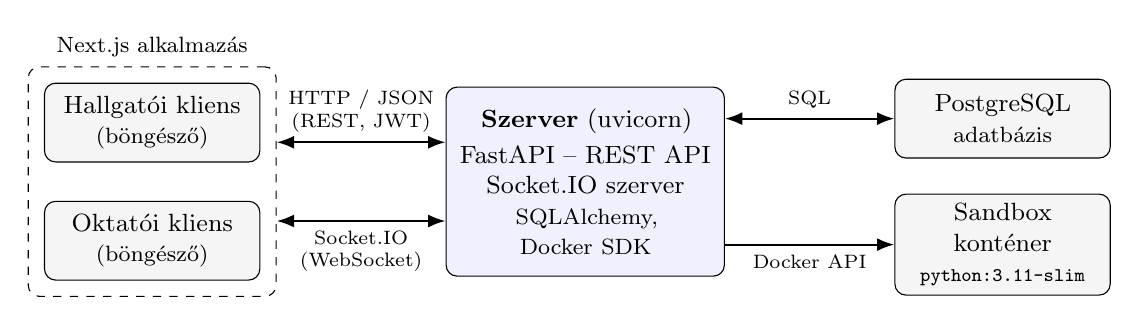
\begin{tikzpicture}[
      box/.style={draw, rounded corners, align=center, minimum height=1.0cm, text width=2.5cm, fill=gray!8, font=\small},
      big/.style={draw, rounded corners, align=center, minimum height=2.4cm, text width=3.3cm, fill=blue!6, font=\small},
      arr/.style={-{Latex[length=2.2mm]}, thick},
      darr/.style={{Latex[length=2.2mm]}-{Latex[length=2.2mm]}, thick},
      lbl/.style={font=\scriptsize, align=center}]
    \node[box] (hallg) at (0,0.75) {Hallgatói kliens\\\footnotesize(böngésző)};
    \node[box] (okt) at (0,-0.75) {Oktatói kliens\\\footnotesize(böngésző)};
    \node[draw, dashed, rounded corners, fit=(hallg)(okt), inner sep=0.2cm,
          label={[font=\footnotesize]above:Next.js alkalmazás}] (front) {};
    \node[big] (back) at (5.5,0) {\textbf{Szerver} (uvicorn)\\[2pt]FastAPI -- REST API\\Socket.IO szerver\\\footnotesize SQLAlchemy, Docker SDK};
    \node[box] (db) at (10.8,0.8) {PostgreSQL\\\footnotesize adatbázis};
    \node[box] (sb) at (10.8,-0.8) {Sandbox konténer\\\scriptsize\texttt{python:3.11-slim}};
    \draw[darr] (front.east |- 0,0.5) -- node[lbl, above]{HTTP / JSON\\(REST, JWT)} (back.west |- 0,0.5);
    \draw[darr] (front.east |- 0,-0.5) -- node[lbl, below]{Socket.IO\\(WebSocket)} (back.west |- 0,-0.5);
    \draw[darr] (back.east |- db.west) -- node[lbl, above]{SQL} (db.west);
    \draw[arr] (back.east |- sb.west) -- node[lbl, below]{Docker API} (sb.west);
  \end{tikzpicture}
  \caption{A rendszer architektúrája}
  \label{fig:architektura}
\end{figure}

A szerver és a kliensek között kétféle kapcsolat létezik. A REST API-n keresztül zajlik minden
olyan művelet, amely az adatok lekérdezésével vagy módosításával jár: a bejelentkezés, a vizsgák
és feladatok kezelése, a válaszok mentése és a kódfuttatás. A Socket.IO kapcsolat kizárólag a
felügyeleti eseményeket továbbítja. Ezt a szétválasztást tudatosan terveztem így: a vizsga
lebonyolításához szükséges összes funkció a valós idejű kapcsolat nélkül is működik, így ha az
például egy hálózati eszköz miatt nem jön létre, a hallgató akkor is zavartalanul kitöltheti a
vizsgát.

A szerveroldali alkalmazást rétegekre bontottam (\mref{tab:retegek}). Az API réteg csak a kérések
fogadásáért, a jogosultság ellenőrzéséért és a válasz összeállításáért felel, az üzleti logika
(a pontozás, a kódfuttatás és a felügyelet) a szolgáltatási rétegben kapott helyet. Ennek
előnye, hogy a pontozási szabályok egy helyen vannak, és több végpont -- a beküldés, a beadás, a
lejárt kitöltések lezárása és az oktatói újraértékelés -- is ugyanazt a kódot használja.

\begin{table}[H]
  \centering
  \caption{A szerveroldali alkalmazás rétegei}
  \label{tab:retegek}
  \begin{tabularx}{\textwidth}{@{}lX@{}}
    \toprule
    Könyvtár & Feladat \\
    \midrule
    \texttt{app/api}      & REST végpontok: hitelesítés, vizsgák és feladatok, kitöltések, eredmények \\
    \texttt{app/schemas}  & Pydantic sémák: a be- és kimenő adatok szerkezete, ellenőrzése, szerepkör szerinti nézetek \\
    \texttt{app/services} & üzleti logika: pontozás, sandbox, Socket.IO események \\
    \texttt{app/models}   & SQLAlchemy ORM modellek (adatbázistáblák) \\
    \texttt{app/core}     & adatbázis-kapcsolat, jelszó- és tokenkezelés, időkezelés \\
    \bottomrule
  \end{tabularx}
\end{table}

\section{Adatmodell}
\label{sec:adatmodell}

Az adatmodell öt entitásból áll, ezek kapcsolatait \aref{fig:adatmodell}. ábra mutatja. A
\texttt{User} a felhasználókat tárolja szerepkörükkel együtt. Az \texttt{Exam} egy vizsgát ír le,
amelyet egy oktató hoz létre, és amelyhez több \texttt{Question}, vagyis feladat tartozik. Az
\texttt{Attempt} egy hallgató egy vizsgakitöltését jelenti a kezdés, a határidő és a befejezés
időpontjával, valamint a felügyelet által rögzített szabálysértések számával. Az \texttt{Answer}
egy kitöltésen belül egy feladatra adott választ és annak értékelését tárolja.

\begin{figure}[H]
  \centering
  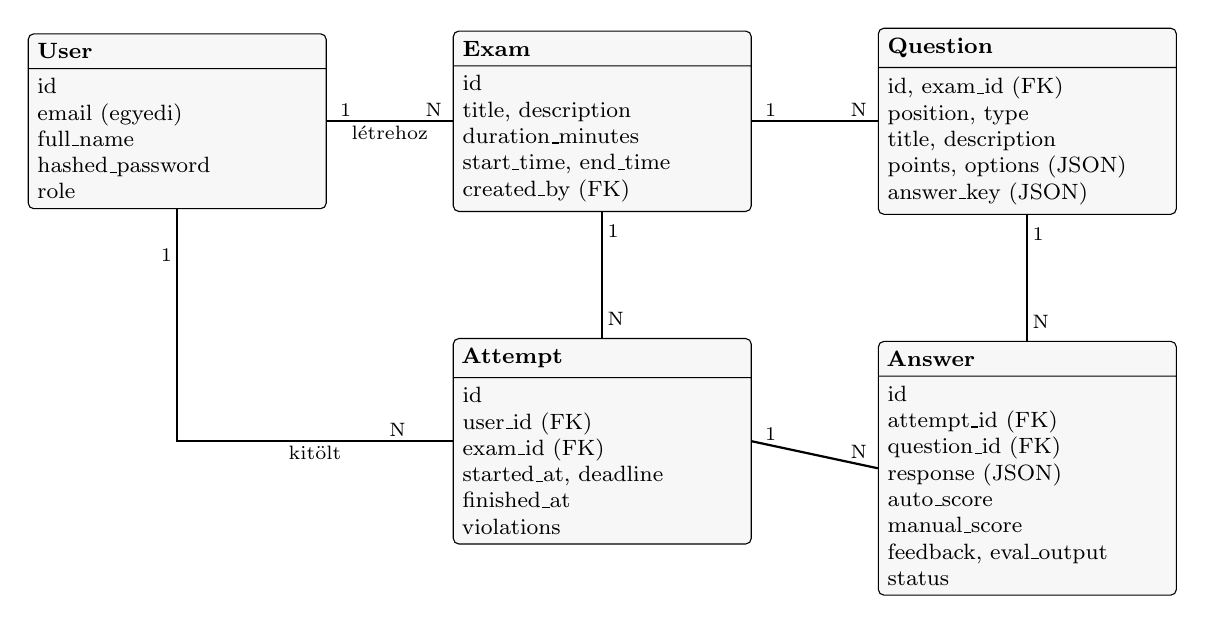
\begin{tikzpicture}[
      ent/.style={rectangle split, rectangle split parts=2, draw, rounded corners=2pt,
                  align=flush left, font=\footnotesize, fill=gray!6, text width=3.55cm,
                  rectangle split part fill={blue!12,gray!4}},
      rel/.style={thick},
      card/.style={font=\scriptsize, inner sep=1.5pt},
      node distance=1.0cm and 1.3cm]
    \node[ent] (user) {\textbf{User}\nodepart{two}id\\email (egyedi)\\full\_name\\hashed\_password\\role};
    \node[ent, right=1.6cm of user] (exam) {\textbf{Exam}\nodepart{two}id\\title, description\\duration\_minutes\\start\_time, end\_time\\created\_by (FK)};
    \node[ent, right=1.6cm of exam] (question) {\textbf{Question}\nodepart{two}id, exam\_id (FK)\\position, type\\title, description\\points, options (JSON)\\answer\_key (JSON)};
    \node[ent, below=1.6cm of exam] (attempt) {\textbf{Attempt}\nodepart{two}id\\user\_id (FK)\\exam\_id (FK)\\started\_at, deadline\\finished\_at\\violations};
    \node[ent, below=1.6cm of question] (answer) {\textbf{Answer}\nodepart{two}id\\attempt\_id (FK)\\question\_id (FK)\\response (JSON)\\auto\_score\\manual\_score\\feedback, eval\_output\\status};
    \draw[rel] (user.east) -- node[card, above, pos=0.15]{1} node[card, above, pos=0.85]{N} node[card, below]{létrehoz} (exam.west);
    \draw[rel] (exam.east) -- node[card, above, pos=0.15]{1} node[card, above, pos=0.85]{N} (question.west);
    \draw[rel] (user.south) |- node[card, left, pos=0.1]{1} node[card, above, pos=0.9]{N} node[card, below, pos=0.75]{kitölt} (attempt.west);
    \draw[rel] (exam.south) -- node[card, right, pos=0.15]{1} node[card, right, pos=0.85]{N} (attempt.north);
    \draw[rel] (attempt.east) -- node[card, above, pos=0.15]{1} node[card, above, pos=0.85]{N} (answer.west);
    \draw[rel] (question.south) -- node[card, right, pos=0.15]{1} node[card, right, pos=0.85]{N} (answer.north);
  \end{tikzpicture}
  \caption{Az adatmodell entitásai és kapcsolataik}
  \label{fig:adatmodell}
\end{figure}

Az adatmodell kialakításakor több fontos tervezési döntést hoztam. Az első a különböző
feladattípusok egységes kezelése. Ahelyett, hogy minden feladattípushoz külön táblát hoztam
volna létre, egyetlen \texttt{Question} táblát használok, amelyben a típusonként eltérő
szerkezetű adatok -- a válaszlehetőségek és a megoldókulcs -- JSON típusú oszlopokba kerülnek
(\mref{tab:megoldokulcs}). Ugyanígy az \texttt{Answer} tábla \texttt{response} oszlopa is JSON:
választós feladatnál a megjelölt lehetőségek indexeinek listáját, a többi feladattípusnál pedig
a válasz szövegét tartalmazza. Ez a megoldás egyszerűvé teszi új feladattípus bevezetését, az
adatok szerkezetének helyességét azonban így nem az adatbázis, hanem az alkalmazás (a Pydantic
sémák) ellenőrzi.

\begin{table}[H]
  \centering
  \caption{A megoldókulcs szerkezete feladattípusonként}
  \label{tab:megoldokulcs}
  \small
  \begin{tabularx}{\textwidth}{@{}lX@{}}
    \toprule
    Feladattípus & A megoldókulcs (\texttt{answer\_key}) tartalma \\
    \midrule
    egyválasztós, igaz--hamis & a helyes válasz indexe egyelemű listában, pl. \texttt{[1]} \\
    több választós            & a helyes válaszok indexeinek listája, pl. \texttt{[0, 1, 3]} \\
    rövid szöveges            & az elfogadott válaszok listája, pl. \texttt{["3.14"]} \\
    programozási              & tesztesetek listája: \texttt{\{input, expected\_output, public\}} \\
    kifejtős                  & nincs (kézi javítás) \\
    \bottomrule
  \end{tabularx}
\end{table}

A második döntés az adatintegritás adatbázis-szintű biztosítása. Az \texttt{Attempt} táblán egy
egyedi megszorítás biztosítja, hogy egy hallgató egy vizsgát csak egyszer töltsön ki, az
\texttt{Answer} táblán pedig egy másik megszorítás azt, hogy egy kitöltésen belül minden
feladatra legfeljebb egy válasz tartozzon. Ezeket a szabályokat az alkalmazás is ellenőrzi, az
adatbázis-szintű megszorítás azonban az egyidejű kérések esetén is garantálja a helyességet.

A harmadik döntés az automatikus és a kézi pontszám külön tárolása. Az \texttt{Answer} rekord
\texttt{auto\_score} mezője a rendszer által számolt, a \texttt{manual\_score} mezője az oktató
által adott pontszámot tartalmazza. Az érvényes pontszám a kézi pontszám, ha az létezik, egyébként
az automatikus. Így az oktatói felülírás bármikor visszavonható, és utólag is ellenőrizhető, mit
számolt a rendszer. A válasz állapotát a \texttt{status} mező tárolja, amelynek lehetséges értékeit
\aref{sec:folyamat}. szakaszban ismertetem.

Végül az időpontokat minden esetben egyezményes világidőben (UTC), időzóna-információval együtt
tárolom, és a kliens csak a megjelenítéskor alakítja át helyi időre. Ez elkerüli a nyári és téli
időszámítás közötti váltásból, valamint a szerver és a kliens eltérő időzónájából adódó hibákat.

\section{A REST API terve}
\label{sec:api}

Az API tervezésénél a REST elveit követtem: az erőforrásokat főnevekből álló URL-ek azonosítják,
a műveleteket a HTTP metódusok fejezik ki. A fontosabb végpontokat \aref{tab:api}. táblázat
tartalmazza. A hallgatói kitöltés indítására a \texttt{POST /exams/\{id\}/attempt} végpontot
terveztem úgy, hogy ismételt hívás esetén ne hozzon létre új kitöltést, hanem a már folyamatban
lévőt adja vissza. Ez a művelet így idempotens, vagyis az oldal frissítése vagy egy megismételt
kérés nem okoz hibát.

\begin{table}[H]
  \centering
  \caption{A REST API fontosabb végpontjai}
  \label{tab:api}
  \small
  \begin{tabularx}{\textwidth}{@{}lp{6.3cm}lX@{}}
    \toprule
    Metódus & Végpont & Jog & Funkció \\
    \midrule
    POST   & \texttt{/auth/register}, \texttt{/auth/login} & -- & regisztráció, bejelentkezés \\
    GET    & \texttt{/exams/} & mindkettő & vizsgák listája \\
    POST   & \texttt{/exams/} & oktató & vizsga létrehozása \\
    POST   & \texttt{/exams/\{id\}/questions} & oktató & feladat hozzáadása \\
    POST   & \texttt{/exams/\{id\}/attempt} & hallgató & kitöltés indítása vagy folytatása \\
    PUT    & \texttt{/attempts/\{id\}/answers/\{qid\}} & hallgató & válasz mentése \\
    POST   & \texttt{/attempts/\{id\}/run} & hallgató & kód próbafuttatása \\
    POST   & \texttt{/attempts/\{id\}/answers/\{qid\}}\newline\texttt{/evaluate} & hallgató & kód beküldése értékelésre \\
    POST   & \texttt{/attempts/\{id\}/finish} & hallgató & végleges beadás \\
    GET    & \texttt{/exams/\{id\}/results(.csv)} & oktató & eredmények, CSV export \\
    PATCH  & \texttt{/answers/\{id\}/grade} & oktató & kézi pontozás, visszajelzés \\
    POST   & \texttt{/exams/\{id\}/regrade} & oktató & sikertelen értékelések újrafuttatása \\
    \bottomrule
  \end{tabularx}
\end{table}

A hibák jelzésére a HTTP szabványos állapotkódjait használom, egységes jelentéssel
(\mref{tab:statuszkodok}). A hibaüzenetek szövege magyar nyelvű, így a kliens azokat
változtatás nélkül megjelenítheti a felhasználónak.

\begin{table}[H]
  \centering
  \caption{A használt hibakódok jelentése}
  \label{tab:statuszkodok}
  \small
  \begin{tabularx}{\textwidth}{@{}lX@{}}
    \toprule
    Kód & Jelentés a rendszerben \\
    \midrule
    400 Bad Request          & hibás kérés, pl. foglalt e-mail cím, érvénytelen meghívókód \\
    401 Unauthorized         & hiányzó, érvénytelen vagy lejárt token, hibás jelszó \\
    403 Forbidden            & nincs jogosultság: más szerepkör, más oktató vizsgája, időablakon kívüli indítás \\
    404 Not Found            & nem létező vagy nem a felhasználóhoz tartozó erőforrás \\
    409 Conflict             & a kitöltés már lezárult (beadva vagy lejárt), módosítás nem lehetséges \\
    422 Unprocessable Entity & a beküldött adatok nem felelnek meg a szabályoknak (validációs hiba) \\
    \bottomrule
  \end{tabularx}
\end{table}

Megemlítendő, hogy ha egy hallgató egy másik hallgató kitöltésére hivatkozik, a szerver nem
\texttt{403}, hanem \texttt{404} választ ad. Ennek az az oka, hogy a \texttt{403} válasz elárulná,
hogy az adott azonosítójú kitöltés létezik, ami -- bár kis mértékben -- információt szivárogtatna
ki a rendszerről.

\section{A vizsgafolyamat terve}
\label{sec:folyamat}

Egy kitöltés életciklusa egyszerű állapotgéppel írható le (\mref{fig:allapotok}). A kitöltés a
vizsga elindításával jön létre, ekkor a szerver kiszámítja a határidőt. Folyamatban lévő
állapotában a hallgató mentheti a válaszait és futtathatja a kódját. A kitöltés kétféleképpen
zárulhat le: a hallgató beadja, vagy lejár a határideje. A lezárás után a válaszok már nem
módosíthatók, a rendszer pedig minden még nem értékelt választ kiértékel.

\begin{figure}[H]
  \centering
  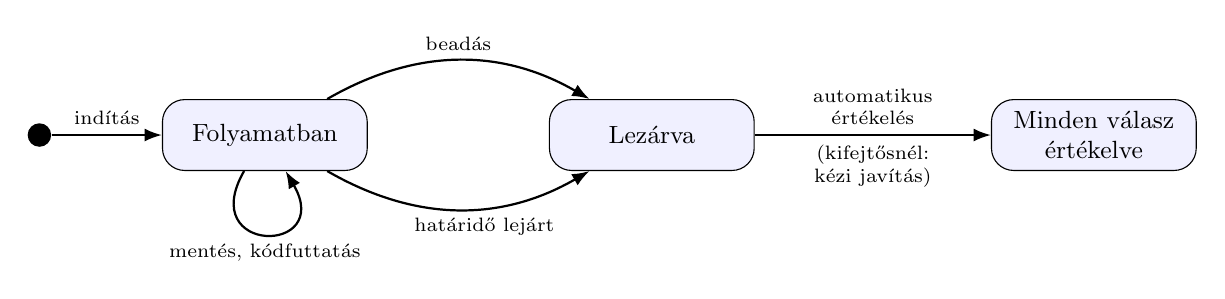
\begin{tikzpicture}[
      st/.style={draw, rounded corners=8pt, align=center, minimum height=0.9cm, minimum width=2.6cm, fill=blue!6, font=\small},
      arr/.style={-{Latex[length=2.2mm]}, thick},
      lbl/.style={font=\scriptsize, align=center},
      node distance=0.9cm and 2.4cm]
    \node[circle, fill=black, inner sep=3pt] (init) {};
    \node[st, right=1.4cm of init] (fut) {Folyamatban};
    \node[st, right=2.3cm of fut] (lez) {Lezárva};
    \node[st, right=3.0cm of lez] (ert) {Minden válasz\\értékelve};
    \draw[arr] (init) -- node[lbl, above]{indítás} (fut);
    \draw[arr] (fut) to[bend left=30] node[lbl, above]{beadás} (lez);
    \draw[arr] (fut) to[bend right=30] node[lbl, below, pos=0.6]{határidő lejárt} (lez);
    \draw[arr] (fut) to[out=-120, in=-60, looseness=6] node[lbl, below]{mentés, kódfuttatás} (fut);
    \draw[arr] (lez) -- node[lbl, above]{automatikus\\értékelés} node[lbl, below]{(kifejtősnél:\\kézi javítás)} (ert);
  \end{tikzpicture}
  \caption{Egy kitöltés állapotai}
  \label{fig:allapotok}
\end{figure}

Az egyes válaszok értékelési állapotát külön mező tárolja, amelynek három értéke lehet.
A \textit{nem értékelt} (\texttt{not\_graded}) állapotú válasz még nem kapott pontszámot: ilyen a
vizsga közben mentett válasz, vagy az a programozási feladat, amelynek értékelése rendszerhiba
miatt nem sikerült. Az \textit{értékelt} (\texttt{graded}) válasz automatikusan vagy kézzel
megkapta a pontszámát. A \textit{javításra váró} (\texttt{pending\_review}) állapotba a kifejtős
válaszok kerülnek a beadáskor, és az oktató pontozásáig ott maradnak. A hallgató a válasz
módosításakor visszakerül a nem értékelt állapotba, így egy korábban beküldött, de azóta
megváltoztatott kód eredménye nem marad érvényben.

A határidő kezelését úgy terveztem, hogy az a szerveren, és ne a kliensen dőljön el. A
határidőt a kitöltés indításakor a szerver számítja ki és tárolja el, a kliens csak megjeleníti.
A lejárt kitöltéseket nem egy időzített háttérfolyamat zárja le, hanem a rendszer minden olyan
kérésnél ellenőrzi és szükség esetén lezárja, amely a kitöltéshez hozzáfér. Ez a ,,lusta''
megközelítés egyszerűbbé teszi a rendszert, hiszen nincs szükség ütemezőre, és a lezárás
eredménye akkor is helyes, ha a szerver a határidő pillanatában éppen nem futott.

\section{A valós idejű felügyelet terve}
\label{sec:felugyelet_terv}

A felügyelet résztvevői a hallgatói kliens, a szerver és az oktatói kliens. A kommunikáció
menetét \aref{fig:szekvencia}. ábra szekvenciadiagramja mutatja be. Mindkét kliens a JWT
tokenjével csatlakozik a szerverhez, majd a \texttt{join\_exam} üzenettel belép a vizsga
szobájába. Az oktató belépéskor egy pillanatképet kap az összes kitöltés aktuális állapotáról, így
a vizsga közben csatlakozva, vagy az oldal frissítése után is teljes képet lát. Ha a hallgató
elhagyja a vizsgaablakot, a kliense \texttt{report\_violation} üzenetet küld, a szerver
eltárolja az eseményt az adatbázisban, majd \texttt{violation\_alert} üzenettel továbbítja a
szoba többi tagjának, vagyis az oktatónak.

\begin{figure}[H]
  \centering
  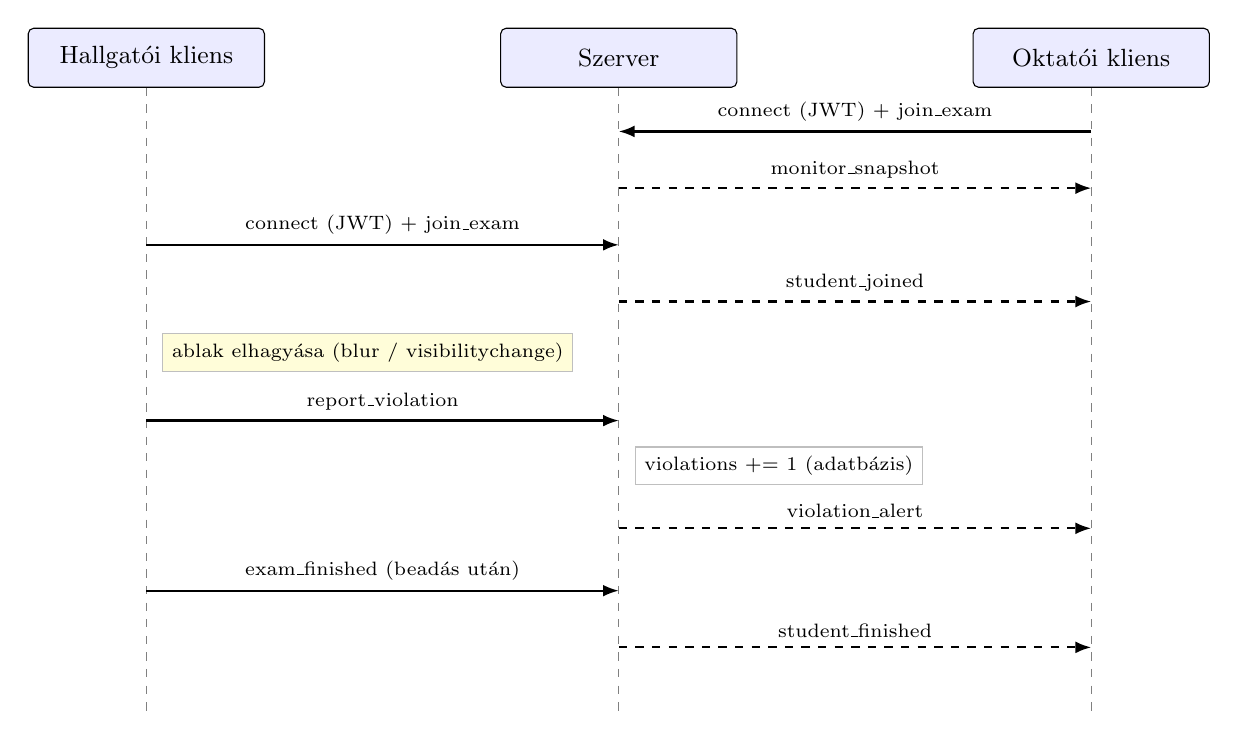
\begin{tikzpicture}[
      head/.style={draw, fill=blue!8, rounded corners=2pt, minimum width=3.0cm, minimum height=0.75cm, font=\small, align=center},
      msg/.style={-{Latex[length=2mm]}, thick},
      ret/.style={-{Latex[length=2mm]}, thick, dashed},
      lbl/.style={font=\scriptsize, above, align=center},
      x=1cm, y=-0.72cm]
    \node[head] (h) at (0,0) {Hallgatói kliens};
    \node[head] (s) at (6,0) {Szerver};
    \node[head] (o) at (12,0) {Oktatói kliens};
    \foreach \n in {h,s,o} \draw[gray, dashed] (\n.south) -- ++(0,11.0);
    \draw[msg] (12,1.3) -- node[lbl]{connect (JWT) + join\_exam} (6,1.3);
    \draw[ret] (6,2.3) -- node[lbl]{monitor\_snapshot} (12,2.3);
    \draw[msg] (0,3.3) -- node[lbl]{connect (JWT) + join\_exam} (6,3.3);
    \draw[ret] (6,4.3) -- node[lbl]{student\_joined} (12,4.3);
    \node[font=\scriptsize, align=left, anchor=west, fill=yellow!15, draw=gray!50] at (0.2,5.2) {ablak elhagyása (blur / visibilitychange)};
    \draw[msg] (0,6.4) -- node[lbl]{report\_violation} (6,6.4);
    \node[font=\scriptsize, fill=white, draw=gray!50, anchor=west] at (6.2,7.2) {violations += 1 (adatbázis)};
    \draw[ret] (6,8.3) -- node[lbl]{violation\_alert} (12,8.3);
    \draw[msg] (0,9.4) -- node[lbl]{exam\_finished (beadás után)} (6,9.4);
    \draw[ret] (6,10.4) -- node[lbl]{student\_finished} (12,10.4);
  \end{tikzpicture}
  \caption{A valós idejű felügyelet üzenetváltásai}
  \label{fig:szekvencia}
\end{figure}

A felügyelet tervezésénél fontos szempont volt, hogy a kliens által küldött adatokban a szerver ne
bízzon meg. A felhasználó nevét és szerepkörét a szerver a token alapján az adatbázisból olvassa
ki, a szobába lépést pedig jogosultsághoz köti: oktató csak a saját vizsgájának szobájába
léphet be, hallgató pedig csak akkor, ha az adott vizsgán folyamatban lévő kitöltése van. A
beadás jelzését (\texttt{exam\_finished}) a szerver csak akkor továbbítja, ha az adatbázis szerint
a kitöltés valóban lezárult.

\section{Biztonsági terv}
\label{sec:biztonsagi_terv}

A tervezés során összegyűjtöttem a rendszert fenyegető főbb veszélyeket, és mindegyikhez
ellenintézkedést rendeltem. Ezeket \aref{tab:fenyegetesek}. táblázat foglalja össze. A
megvalósítás részleteit \aref{ch:megvalositas}. fejezetben, a védelmek ellenőrzését pedig
\aref{ch:teszteles}. fejezetben mutatom be.

\begin{longtable}{@{}>{\raggedright\arraybackslash}p{5.2cm}>{\raggedright\arraybackslash}p{8.8cm}@{}}
  \caption{Fenyegetések és ellenintézkedések}\label{tab:fenyegetesek}\\
  \toprule
  Fenyegetés & Ellenintézkedés \\
  \midrule
  \endfirsthead
  \toprule
  Fenyegetés & Ellenintézkedés \\
  \midrule
  \endhead
  Jogosulatlan oktatói regisztráció & meghívókód, időzítéses támadásnak ellenálló összehasonlítással \\
  Jelszavak kiszivárgása adatbázis-incidens esetén & bcrypt hash egyedi sóval \\
  Más felhasználó adatainak elérése & szerepkör- és tulajdonjog-ellenőrzés minden végponton; idegen kitöltésre 404 válasz \\
  A megoldókulcs megszerzése & külön hallgatói és oktatói adatséma; a rejtett tesztek részletei nem kerülnek a visszajelzésbe \\
  Határidő utáni módosítás & a határidőt a szerver érvényesíti; lezárt kitöltés nem módosítható (409) \\
  Többszöri kitöltés & egyedi megszorítás az adatbázisban (hallgató, vizsga) \\
  Ártó kód futtatása (erőforrás-kimerítés, fájl- és hálózati hozzáférés) & Docker konténer: memória-, CPU-, folyamat-, idő- és kimenetkorlát; hálózat nélkül; csak olvasható fájlrendszer \\
  Az értékelés eredményének meghamisítása & a hallgató kódja jogosultság nélküli felhasználóként, külön folyamatban fut; a kimenetét a vezérlő gyűjti \\
  Hamis felügyeleti események, más szobájába lépés & JWT-hitelesítés csatlakozáskor; a szerepkör az adatbázisból; szobába lépés jogosultsághoz kötve \\
  \bottomrule
\end{longtable}

%!TEX root = ../dolgozat.tex
\chapter{Megvalósítás}
\label{ch:megvalositas}

Ebben a fejezetben \mref{ch:tervezes}ben ismertetett terv megvalósítását mutatom be.
A teljes forráskódot nem másolom be a dolgozatba, az a mellékelt adathordozón megtalálható;
a fejezetben azokra a részekre koncentrálok, amelyek a megvalósítás során érdemi döntést
vagy technikai nehézséget jelentettek. A rendszer két önálló alkalmazásból áll: egy Python
nyelvű, FastAPI keretrendszerre épülő szerveroldali alkalmazásból és egy Next.js alapú
kliensoldali alkalmazásból, amelyeket egy PostgreSQL adatbázis és a programkódok futtatására
szolgáló Docker-környezet egészít ki.

\section{A szerveroldal felépítése}

A szerveroldali alkalmazás szerkezetét a felelősségi körök szerint alakítottam ki, így az
egyes rétegek egymástól jól elkülönülnek. Az \texttt{app/models} könyvtár tartalmazza az
SQLAlchemy ORM-modelleket \cite{sqlalchemy_docs}, vagyis az adatbázis-táblák Python
osztályként megfogalmazott leírását. Az \texttt{app/schemas} könyvtárban találhatók a Pydantic
sémák, amelyek a REST API-n be- és kimenő adatok szerkezetét írják le és ellenőrzik. Az
\texttt{app/api} könyvtár négy modulja (\texttt{auth}, \texttt{exams}, \texttt{attempts},
\texttt{results}) tartalmazza a végpontokat, míg az \texttt{app/services} könyvtárban kapott
helyet az üzleti logika: a pontozás (\texttt{grading.py}), a kódfuttatás (\texttt{sandbox.py})
és a valós idejű kommunikáció (\texttt{socket\_server.py}). Az \texttt{app/core} könyvtár az
adatbázis-kapcsolatot, a jelszó- és tokenkezelést, valamint az időzónák egységes kezelését
végző segédfüggvényeket foglalja magában.

A FastAPI egyik legnagyobb előnyének a függőséginjektálást (\textit{dependency injection})
tartom \cite{fastapi_docs}. Az adatbázis-munkamenetet egy \texttt{get\_db} nevű generátorfüggvény
állítja elő, amely a kérés végén automatikusan le is zárja a kapcsolatot, így egyetlen
végpontban sem kell erről külön gondoskodni. Ugyanezt a mechanizmust használtam a
jogosultságkezelésre is: a \texttt{require\_teacher} és a \texttt{require\_student} függőségek
a végpont futása előtt ellenőrzik a bejelentkezett felhasználó szerepkörét, és szükség esetén
\texttt{403 Forbidden} választ adnak. Így a jogosultsági szabályok egy helyen vannak megfogalmazva,
és a végpontok törzsében már csak a tényleges feladat logikája szerepel.

Az alkalmazás belépési pontja a \texttt{main.py}, ahol a FastAPI alkalmazást és a Socket.IO
szervert egyetlen ASGI alkalmazássá fűzöm össze. A \texttt{/socket.io} útvonalra érkező
kéréseket a Socket.IO szerver, minden mást a FastAPI kezel, így a két szolgáltatás ugyanazon a
porton, egyetlen \texttt{uvicorn} folyamatban fut. A fejlesztés során gyakran változott az
adatmodell, ezért készítettem egy egyszerű sémaszinkronizáló függvényt
(\texttt{sync\_missing\_columns}), amely induláskor a modellben már szereplő, de az adatbázisból
még hiányzó oszlopokat és egyedi megszorításokat adatvesztés nélkül pótolja. Éles rendszerben
erre a célra egy migrációs eszköz (például az Alembic) volna a megfelelő választás, a prototípus
szintjén azonban ez a megoldás elegendőnek bizonyult.

\section{Hitelesítés és jogosultságkezelés}

A felhasználók jelszavát a rendszer soha nem tárolja nyílt szövegként: regisztrációkor a
\texttt{passlib} könyvtár bcrypt algoritmussal sózott hash-t képez belőle
\cite{provos1999bcrypt}, bejelentkezéskor pedig ezzel hasonlítja össze a megadott jelszót. A
bcrypt előnye, hogy szándékosan lassú, és a munkatényezője növelhető, így a nyers erővel történő
jelszótörés költsége a hardverek fejlődésével együtt emelhető.

Sikeres bejelentkezés után a szerver egy JSON Web Tokent (JWT) állít ki \cite{rfc7519}, amely a
felhasználó e-mail címét és a lejárati időt tartalmazza, és HS256 algoritmussal, a szerver titkos
kulcsával van aláírva. A token egy napig érvényes; a kliens minden további kérésnél az
\texttt{Authorization: Bearer} fejlécben küldi vissza. A JWT előnye, hogy a szervernek nem kell
munkamenet-állapotot tárolnia: az aláírás ellenőrzésével eldönthető, hogy a token hiteles-e. A
szerepkört szándékosan nem a tokenbe írtam, hanem minden kérésnél az adatbázisból olvasom ki,
így egy szerepkör-módosítás azonnal érvényre jut.

Az oktatói regisztrációt meghívókódhoz kötöttem, hiszen ellenkező esetben bármely hallgató
oktatóként regisztrálhatna, és hozzáférhetne a vizsgák megoldókulcsaihoz. A meghívókód
ellenőrzésénél a \texttt{hmac.compare\_digest} függvényt használtam a szokásos egyenlőségvizsgálat
helyett, mert ez az összehasonlítást a bemenettől független idő alatt végzi el, így időzítéses
támadással (\textit{timing attack}) sem lehet a kódot karakterenként kitalálni.

A jogosultságkezelés másik fontos eleme a tulajdonjog ellenőrzése. Egy oktató csak a saját
maga által létrehozott vizsgát tekintheti meg, módosíthatja és értékelheti; ezt a
\texttt{get\_owned\_exam} segédfüggvény biztosítja, amelyet minden oktatói végpont meghív.
A hallgatók hasonlóképpen kizárólag a saját kitöltésükhöz férnek hozzá.

\section{A megoldókulcs védelme}

A rendszer tervezésekor az egyik legfontosabb követelmény az volt, hogy a megoldókulcs semmilyen
módon ne juthasson el a hallgatóhoz (lásd \aref{sec:kovetelmenyek}. szakaszt). Ezt a Pydantic
sémák szintjén oldottam meg: a feladatoknak két külön nézete van. A \texttt{QuestionPublic}
séma csak a feladat szövegét, pontértékét, a válaszlehetőségeket és a kódfeladatok nyilvános
példatesztjeit tartalmazza, míg az ebből származtatott \texttt{QuestionTeacher} séma ezt a
megoldókulccsal egészíti ki. Mivel a FastAPI a válasz előállításakor mindig a végponthoz rendelt
séma mezőit szerializálja, a hallgatói végpontok akkor sem adhatnák ki a megoldókulcsot, ha az
az objektumban egyébként jelen van.

Ugyanez a gondolat érvényesül a vizsga folyamata közben is. A hallgató a feladatokat csak a vizsga
elindításakor kapja meg, a vizsgalistában csak a vizsga címe, időpontja és a feladatok száma
látszik. A pontszámokat és az oktatói visszajelzéseket a szerver csak a beadás után küldi el, a
kódfeladatok rejtett teszteseteiről pedig a hallgató csak annyit tud meg, hogy sikeresek voltak-e;
a bemenetüket, az elvárt kimenetüket és az esetleges hibaüzenetet nem.

\section{A vizsgafolyamat és az időkezelés}

A vizsgafolyamat a hallgató szemszögéből három lépésből áll: elindítja a vizsgát, kitölti a
feladatokat, majd beadja a megoldását. Az indításkor a szerver létrehoz egy kitöltést
(\texttt{Attempt}), és kiszámítja annak határidejét. A vizsgának van egy időablaka (kezdési és
záró időpont), valamint egy időtartama; a hallgató rendelkezésére álló idő e kettő közül a
szigorúbb:
\begin{equation}
  t_{\text{határidő}} = \min\left(t_{\text{vizsga vége}},\ t_{\text{kezdés}} + \Delta t_{\text{időtartam}}\right).
  \label{eq:hatarido}
\end{equation}
Így ha valaki a vizsgaablak vége előtt tíz perccel kezd hozzá egy hatvanperces vizsgához, akkor
is csak tíz perce marad, ami megfelel a hagyományos vizsgák gyakorlatának.

Az adatbázisban a kitöltésekre egyedi megszorítás vonatkozik a hallgató és a vizsga azonosítójára,
vagyis minden hallgató egy vizsgát csak egyszer tölthet ki. Ez a megszorítás egy versenyhelyzetet
is kezel: ha a kliens két indítási kérést küld szinte egyszerre (például dupla kattintás miatt),
akkor a második beszúrás \texttt{IntegrityError} kivétellel meghiúsul, a szerver pedig ilyenkor
visszagörgeti a tranzakciót, és a már létrejött kitöltést adja vissza.

A határidő betartását a szerver ellenőrzi, a kliens oldali visszaszámláló csupán tájékoztató
jellegű. Minden módosító kérésnél (válasz mentése, kód futtatása) az \texttt{is\_active} függvény
megvizsgálja, hogy a kitöltés még nyitott-e. A hálózati késleltetés miatt 30 másodperces türelmi
időt hagytam, hogy az utolsó pillanatban elküldött mentés ne vesszen el. Lejárt kitöltés esetén
a szerver \texttt{409 Conflict} választ ad, és lezárja a kitöltést. A lezárást nem egy külön
időzített folyamat végzi, hanem ,,lusta'' módon történik: bármely végpont, amely a kitöltéshez
hozzáfér (a hallgatói nézet, a hallgató eredménylistája vagy az oktatói eredményoldal), először
meghívja a \texttt{finalize\_if\_expired} függvényt. Ennek az az előnye, hogy nincs szükség
háttérfolyamatra, és a lejárt kitöltések akkor is lezárulnak, ha a hallgató egyszerűen bezárta a
böngészőt.

A kliens oldalon két megoldás teszi megbízhatóvá a kitöltést. Az egyik az automatikus mentés:
a válasz minden módosítás után 800 milliszekundumos késleltetéssel (\textit{debounce}) mentődik,
így gépelés közben nem keletkezik fölösleges hálózati forgalom, a hallgató mégsem veszít el
munkát. A még el nem mentett válaszok miatt a böngésző figyelmeztet, ha a hallgató el akarja
hagyni az oldalt, beadáskor pedig a kliens először minden függőben lévő mentést elküld. A másik
megoldás az óraeltérés kezelése. A hallgató számítógépének órája eltérhet a szerverétől, ezért a
szerver minden válaszában elküldi a saját aktuális idejét, a kliens pedig ebből kiszámítja az
eltérést, és a visszaszámlálót ezzel korrigálja. Amikor a hátralévő idő elfogy, a kliens
automatikusan beadja a vizsgát.

\section{Az automatikus pontozás}
\label{sec:pontozas}

A pontozás logikáját a \texttt{grading.py} modulban, feladattípusonként külön valósítottam meg.
Az egyválasztós és az igaz--hamis feladatoknál a hallgató akkor kapja meg a teljes pontszámot, ha
a megjelölt válasza megegyezik a helyessel. A több helyes választ is tartalmazó feladatoknál a
puszta egyezés túl szigorú volna, a helyes jelölések egyszerű megszámolása viszont lehetővé tenné,
hogy valaki minden lehetőséget megjelöljön. Ezért a rendszer részpontot ad, de a hibás jelöléseket
levonja:
\begin{equation}
  P = \max\!\left(0,\ \frac{|S \cap H| - |S \setminus H|}{|H|}\right) \cdot P_{\max},
  \label{eq:tobbvalasz}
\end{equation}
ahol $S$ a megjelölt, $H$ a helyes válaszok halmaza, $P_{\max}$ pedig a feladat pontértéke. Ha
például három helyes válaszból a hallgató kettőt és egy hibásat jelöl meg, akkor a pontszám
$(2-1)/3$, vagyis a maximális pontszám egyharmada. A nullánál húzott alsó korlát miatt egy feladat
negatív pontot nem eredményezhet.

A rövid szöveges válaszoknál az oktató több elfogadott választ is megadhat. Az összehasonlítás előtt
a rendszer mindkét oldalt normalizálja: kisbetűssé alakítja (a Unicode szerinti
\texttt{casefold} művelettel, amely az ékezetes betűket is helyesen kezeli), és a többszörös
szóközöket egyetlen szóközre cseréli. Ha mindkét érték számként értelmezhető, akkor a rendszer a
számértékeket hasonlítja össze, így a magyar és az angol tizedesjelölés (\texttt{3,14} és
\texttt{3.14}) egyaránt elfogadott. A kifejtős feladatok értelemszerűen nem pontozhatók
automatikusan; ezek beadás után ,,javításra vár'' állapotba kerülnek, és az oktató értékeli őket.

A kézi értékelés minden feladattípusnál elérhető: az oktató felülírhatja az automatikus pontszámot,
és szöveges visszajelzést fűzhet a válaszhoz. Az adatmodellben ezért külön mező tárolja az
automatikus és a kézi pontszámot; ha kézi pontszám létezik, az az érvényes. Ennek köszönhetően a
felülírás visszavonható, és utólag is látszik, mit számolt a rendszer.

\section{Biztonságos kódfuttatás Docker-sandboxban}
\label{sec:sandbox}

A programozási feladatok értékelése a rendszer legérzékenyebb része, hiszen a szerver ilyenkor
egy ismeretlen személy által írt, tetszőleges programkódot futtat. Egy rosszindulatú (vagy
egyszerűen hibás) program megpróbálhat fájlokat olvasni a szerverről, hálózati kapcsolatot
nyitni, elfogyasztani a memóriát, vagy végtelen számú folyamatot indítani. Ezért a kódot
Docker-konténerben futtatom \cite{merkel2014docker}, amelyre szigorú korlátozásokat alkalmazok.
Ezeket \aref{tab:sandbox}. táblázat foglalja össze, a konténer indítási paramétereit pedig
\aref{py:sandbox}. programkód mutatja.

\begin{table}[H]
  \centering
  \caption{A sandbox konténer korlátozásai}
  \label{tab:sandbox}
  \begin{tabularx}{\textwidth}{@{}lX@{}}
    \toprule
    Korlátozás & Érték, cél \\
    \midrule
    Hálózat             & nincs -- adatszivárgás és külső támadás ellen \\
    Memória             & 128 MB \\
    CPU                 & 0,5 mag \\
    Folyamatok száma    & legfeljebb 64 (\enquote{fork bomb} ellen) \\
    Fájlrendszer        & csak olvasható; \texttt{/tmp}: 16 MB-os tmpfs \\
    Jogosultságok       & minden capability eldobva, \texttt{no-new-privileges}; a kód \texttt{nobody}-ként fut \\
    Időkorlát           & 5 mp tesztesetenként \\
    Kimenet             & legfeljebb 64 KB tesztesetenként \\
    \bottomrule
  \end{tabularx}
\end{table}

\begin{python}[caption={A sandbox konténer indítási paraméterei (\texttt{sandbox.py}, részlet)},label=py:sandbox]
run_kwargs = dict(
    image=SANDBOX_IMAGE,
    command=["python", "-c", _RUNNER],
    network_mode="none",
    mem_limit="128m",
    nano_cpus=500_000_000,
    pids_limit=64,
    read_only=True,
    tmpfs={"/tmp": "size=16m,mode=1777"},
    cap_drop=["ALL"],
    cap_add=["SETUID", "SETGID", "KILL"],
    security_opt=["no-new-privileges"],
)
\end{python}

Az első változatban minden tesztesethez külön konténert indítottam, ez azonban egy tíz tesztesetből
álló feladatnál már több másodperces várakozást jelentett, mivel a konténer indítása önmagában is
időigényes. Ezért a végleges megoldásban egy kiértékeléshez egyetlen konténer indul, amelyben egy
rövid vezérlőprogram (\textit{runner}) egymás után futtatja le a hallgató kódját az összes
tesztbemenettel, majd az eredményeket JSON formátumban adja vissza. A konténer indításának
költsége így csak egyszer jelentkezik.

Ez a megoldás azonban felvet egy újabb biztonsági kérdést: ha a hallgató kódja ugyanabban a
környezetben fut, mint a vezérlőprogram, akkor elvileg meghamisíthatná az eredményeket. Ezt úgy
zártam ki, hogy a vezérlőprogram rendszergazdai jogokkal fut, a hallgató kódját viszont egy
alfolyamatban, a jogosultságokkal nem rendelkező \texttt{nobody} felhasználóként (65534-es
azonosító) indítja el. A hallgató programjának szabványos kimenetét a vezérlőprogram csövön
(\textit{pipe}) keresztül olvassa be, így az nem keveredhet a vezérlőprogram saját kimenetével.
Ehhez kellett a \texttt{SETUID} és \texttt{SETGID} képességeket meghagyni a konténerben, a
\texttt{KILL} képességre pedig azért volt szükség, hogy az időtúllépés esetén a vezérlőprogram a
hallgató folyamatát -- az általa esetleg indított gyermekfolyamatokkal együtt -- le tudja állítani.
A \texttt{no-new-privileges} beállítás biztosítja, hogy a hallgató kódja semmilyen módon ne
szerezhessen vissza magasabb jogosultságot.

A kimenet olvasását külön szálak végzik, amelyek a megadott korlát (64 KB) fölötti részt eldobják.
Erre azért van szükség, mert egy végtelen ciklusban kiíró program néhány másodperc alatt is
gigabájtos kimenetet képes előállítani, ami a szerver memóriáját terhelné. A hallgató kódját és a
tesztbemeneteket környezeti változókban adom át a konténernek, nem pedig csatolt könyvtárban
(\textit{volume}). Ezt a döntést gyakorlati tapasztalat indokolta: Windows és Docker Desktop alatt
a könyvtárcsatolás lassú és megbízhatatlan volt, a környezeti változós átadás viszont minden
platformon egyformán működik.

A tesztek kiértékelésekor a rendszer a program kimenetét a sor eleji és végi szóközök levágása
után hasonlítja össze az elvárt kimenettel, és csak akkor tekinti a tesztet sikeresnek, ha a
program hiba nélkül (nulla kilépési kóddal) és időkorláton belül futott le. A pontszám a sikeres
tesztek arányával arányos. Fontos szempont volt az is, hogy rendszerhiba (például ha a Docker
szolgáltatás éppen nem fut) esetén a hallgató ne kapjon nulla pontot: ilyenkor a válasz
,,nem értékelt'' állapotban marad, az oktató pedig a hiba elhárítása után egyetlen gombnyomással
újraértékelheti a vizsga összes ilyen válaszát.

A hallgató a vizsga közben kétféleképpen futtathatja a kódját. A próbafuttatás saját bemenettel
vagy a nyilvános példatesztekkel fut le, és nem befolyásolja a pontszámot; ez a fejlesztői
környezetekben megszokott ,,futtatás'' gombnak felel meg. A beküldés ezzel szemben az összes, a
rejtett teszteseteket is tartalmazó tesztkészlettel értékeli a megoldást, és elmenti az eredményt.

\section{Valós idejű felügyelet}

A felügyeleti funkció célja, hogy az oktató a vizsga ideje alatt azonnal értesüljön, ha egy hallgató
elhagyja a vizsgaablakot, például egy másik böngészőfülre vált vagy másik alkalmazást nyit meg. A
kliens oldalon ezt a \texttt{useProctoring} nevű React hook valósítja meg, amely a böngésző két
eseményére iratkozik fel: az ablak fókuszvesztésére (\texttt{blur}) és a lap láthatóságának
megváltozására (\texttt{visibilitychange}). Fülváltáskor a böngésző mindkét eseményt kiváltja,
ezért egy egyszerű jelzővel biztosítottam, hogy egy elhagyás csak egyszer számítson; a jelző az
ablak visszakapott fókuszakor áll vissza (\aref{ts:proctoring}. programkód).

\begin{typescript}[caption={Az ablakelhagyás érzékelése (\texttt{useProctoring.ts}, részlet)},label=ts:proctoring]
let away = false;
const handleBlur = () => {
  if (away) return;
  away = true;
  report('WINDOW_BLUR (ablakfókusz elvesztve)');
};
const handleFocus = () => { away = false; };
const handleVisibility = () => {
  if (document.visibilityState === 'hidden' && !away) {
    away = true;
    report('TAB_HIDDEN (lapváltás / kis méret)');
  }
};
\end{typescript}

A kommunikációhoz a Socket.IO könyvtárat használtam \cite{socketio_docs}, amely WebSocket
kapcsolatot épít ki \cite{rfc6455}, de annak elérhetetlensége esetén más átviteli módra is képes
visszaváltani, és beépítetten támogatja az újracsatlakozást és a szobákat (\textit{rooms}).
Minden vizsgához tartozik egy szoba, ebbe lépnek be a vizsgázó hallgatók és a vizsgát felügyelő
oktató. Csatlakozáskor a kliens elküldi a JWT tokenjét, amelyet a szerver ugyanúgy ellenőriz, mint
a REST API esetén; érvénytelen tokennel a kapcsolat létre sem jön. A felhasználó nevét és
szerepkörét a szerver az adatbázisból olvassa ki, nem a klienstől fogadja el, így a hallgató nem
adhatja ki magát oktatónak. A szobába lépésnél a szerver további ellenőrzést végez: oktató csak a
saját vizsgája szobájába léphet be, hallgató pedig csak akkor, ha az adott vizsgán folyamatban lévő
kitöltése van.

Amikor a hallgató kliense szabálysértést jelez, a szerver megnöveli a kitöltéshez tartozó
számlálót az adatbázisban, majd továbbítja az eseményt a szoba többi résztvevőjének, vagyis az
oktatónak. Azért döntöttem az adatbázisban való tárolás mellett, mert így a számláló nem vész el,
ha a hallgató frissíti az oldalt, vagy ha az oktató később csatlakozik: belépéskor az oktató
pillanatképet (\textit{snapshot}) kap a vizsga összes kitöltésének aktuális állapotáról, és a
szabálysértések száma az eredménylistában és a CSV exportban is megjelenik. Mivel a Socket.IO
szerver aszinkron módon működik, az SQLAlchemy szinkron adatbázis-műveletei viszont blokkolnák az
eseményhurkot, ezeket az \texttt{asyncio.to\_thread} függvénnyel külön szálon futtatom. A szerver
azt is nyilvántartja, hogy egy hallgató hány böngészőfülön csatlakozik, így az oktató csak akkor
látja ,,offline'' állapotúnak, ha az összes kapcsolata megszakadt.

Fontosnak tartom kiemelni, hogy ez a megoldás nem nyújt teljes védelmet a csalás ellen: egy
második eszközt (például mobiltelefont) használó hallgatót a böngésző nem képes érzékelni. A
funkció célja inkább a visszatartás és az oktató tájékoztatása; a webkamerás vagy
mesterséges intelligenciára épülő felügyelet \mref{ch:koncepcio}ben bemutatott adatvédelmi és
etikai kérdések miatt nem volt célja ennek a dolgozatnak.

\section{A felhasználói felület}
\label{sec:felulet}

A kliensoldali alkalmazást a Next.js keretrendszer App Router megoldásával készítettem
\cite{nextjs_docs}, a megjelenéshez a Tailwind CSS segédosztályait használtam. Az oldalak a
szerepkörök szerint két csoportra oszlanak. A hallgatói műszerfalon a hallgató látja az elérhető
vizsgákat és a korábbi eredményeit. A vizsgaoldal rögzített fejlécében a hátralévő idő, a
felügyeleti kapcsolat állapota és az ablakváltások száma látható, a feladatok között pedig egy
gombsorban navigálhat, ahol pipa jelzi, mely feladatokra válaszolt már; az éppen szerkesztett
feladatnál az automatikus mentés állapota (,,Mentés\ldots'', ,,Mentve'') is megjelenik. Az oktatói felületen a vizsgák kezelése mellett egy vizsgához három fül tartozik: a
feladatszerkesztő, az élő monitor és az eredmények.

A feladatszerkesztő típusonként eltérő űrlapot jelenít meg: választós feladatnál a
válaszlehetőségek és a helyes válaszok megjelölése, rövid válasznál az elfogadott válaszok,
kódfeladatnál pedig a tesztesetek szerkesztése jelenik meg, ahol minden tesztesetről megadható,
hogy nyilvános példateszt vagy rejtett teszt legyen. Az űrlapon megadott adatokat a szerver a
Pydantic sémákban megfogalmazott szabályok szerint is ellenőrzi és egységes formára hozza, így
hibás megoldókulcs (például nem létező válaszlehetőségre mutató index) nem kerülhet az
adatbázisba.

Az eredmények fülön az oktató hallgatónként áttekintheti a válaszokat, pontozhatja a kifejtős
feladatokat, és az eredményeket CSV fájlba exportálhatja. Az export kialakításánál a magyar
nyelvű Excel sajátosságaihoz igazodtam: pontosvesszőt használtam elválasztóként, és a fájl elejére
UTF-8 bájtsorrend-jelzőt (BOM) írtam, mert enélkül az Excel hibásan jeleníti meg az ékezetes
karaktereket.

A programkód szerkesztésére egy egyszerű, egyenközű betűtípussal megjelenített szövegmezőt
használtam. Egy fejlettebb, szintaxiskiemelést nyújtó szerkesztő (például a Monaco Editor)
beépítése kényelmesebbé tenné a munkát, ezt a továbbfejlesztési lehetőségek között tartom számon.

A hallgatói vizsgaoldalt programozási feladat közben \aref{fig:vizsgaoldal_kod}. ábra mutatja. A
fejlécben a visszaszámláló, a felügyelet állapota és az ablakváltások száma látható, alatta a
feladatok gombsora. A feladat szövege alatt a nyilvános példatesztek jelennek meg, a bal oldali
szerkesztőben a hallgató a kódját írja, a jobb oldali konzolban pedig a próbafuttatás és az utolsó
beküldés értékelésének eredménye látható.

\begin{figure}[H]
  \centering
  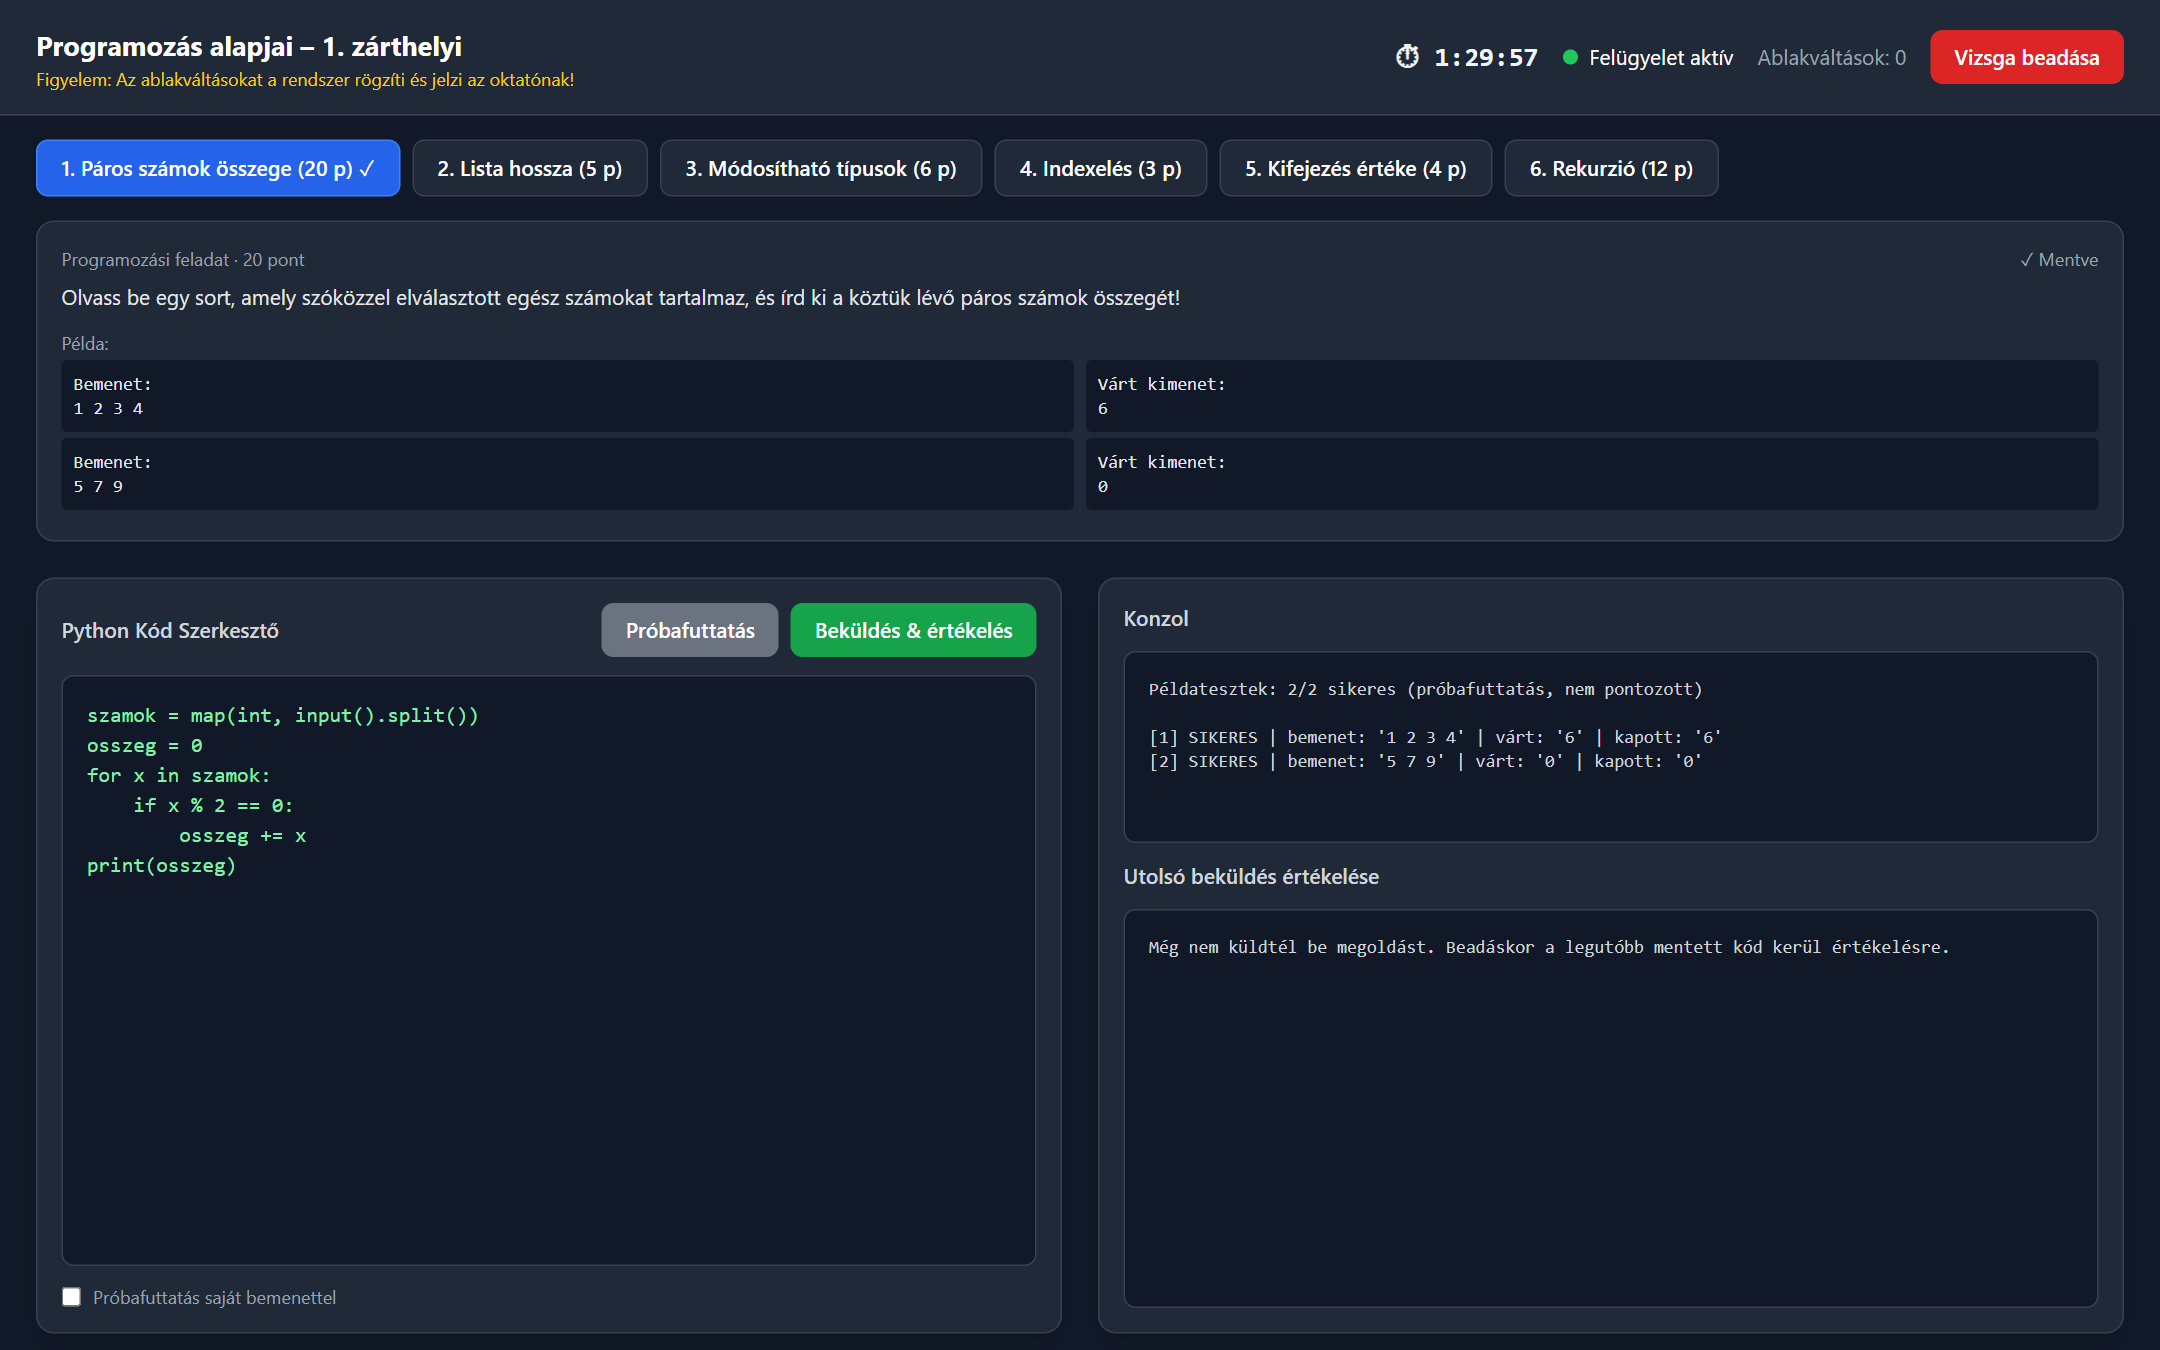
\includegraphics[width=\textwidth]{images/vizsgaoldal_kod.png}
  \caption{A hallgatói vizsgaoldal programozási feladattal, sikeres próbafuttatás után}
  \label{fig:vizsgaoldal_kod}
\end{figure}

Az oktatói feladatszerkesztőt \aref{fig:feladatszerkeszto}. ábra mutatja. A bal oldalon a vizsga
már felvett feladatai láthatók a megoldókulccsal együtt (a helyes válaszokat pipa jelöli), a jobb
oldali űrlap pedig a kiválasztott típushoz igazodik; az ábrán egy programozási feladat
tesztesetének megadása látható, a ,,nyilvános'' jelölővel.

\begin{figure}[H]
  \centering
  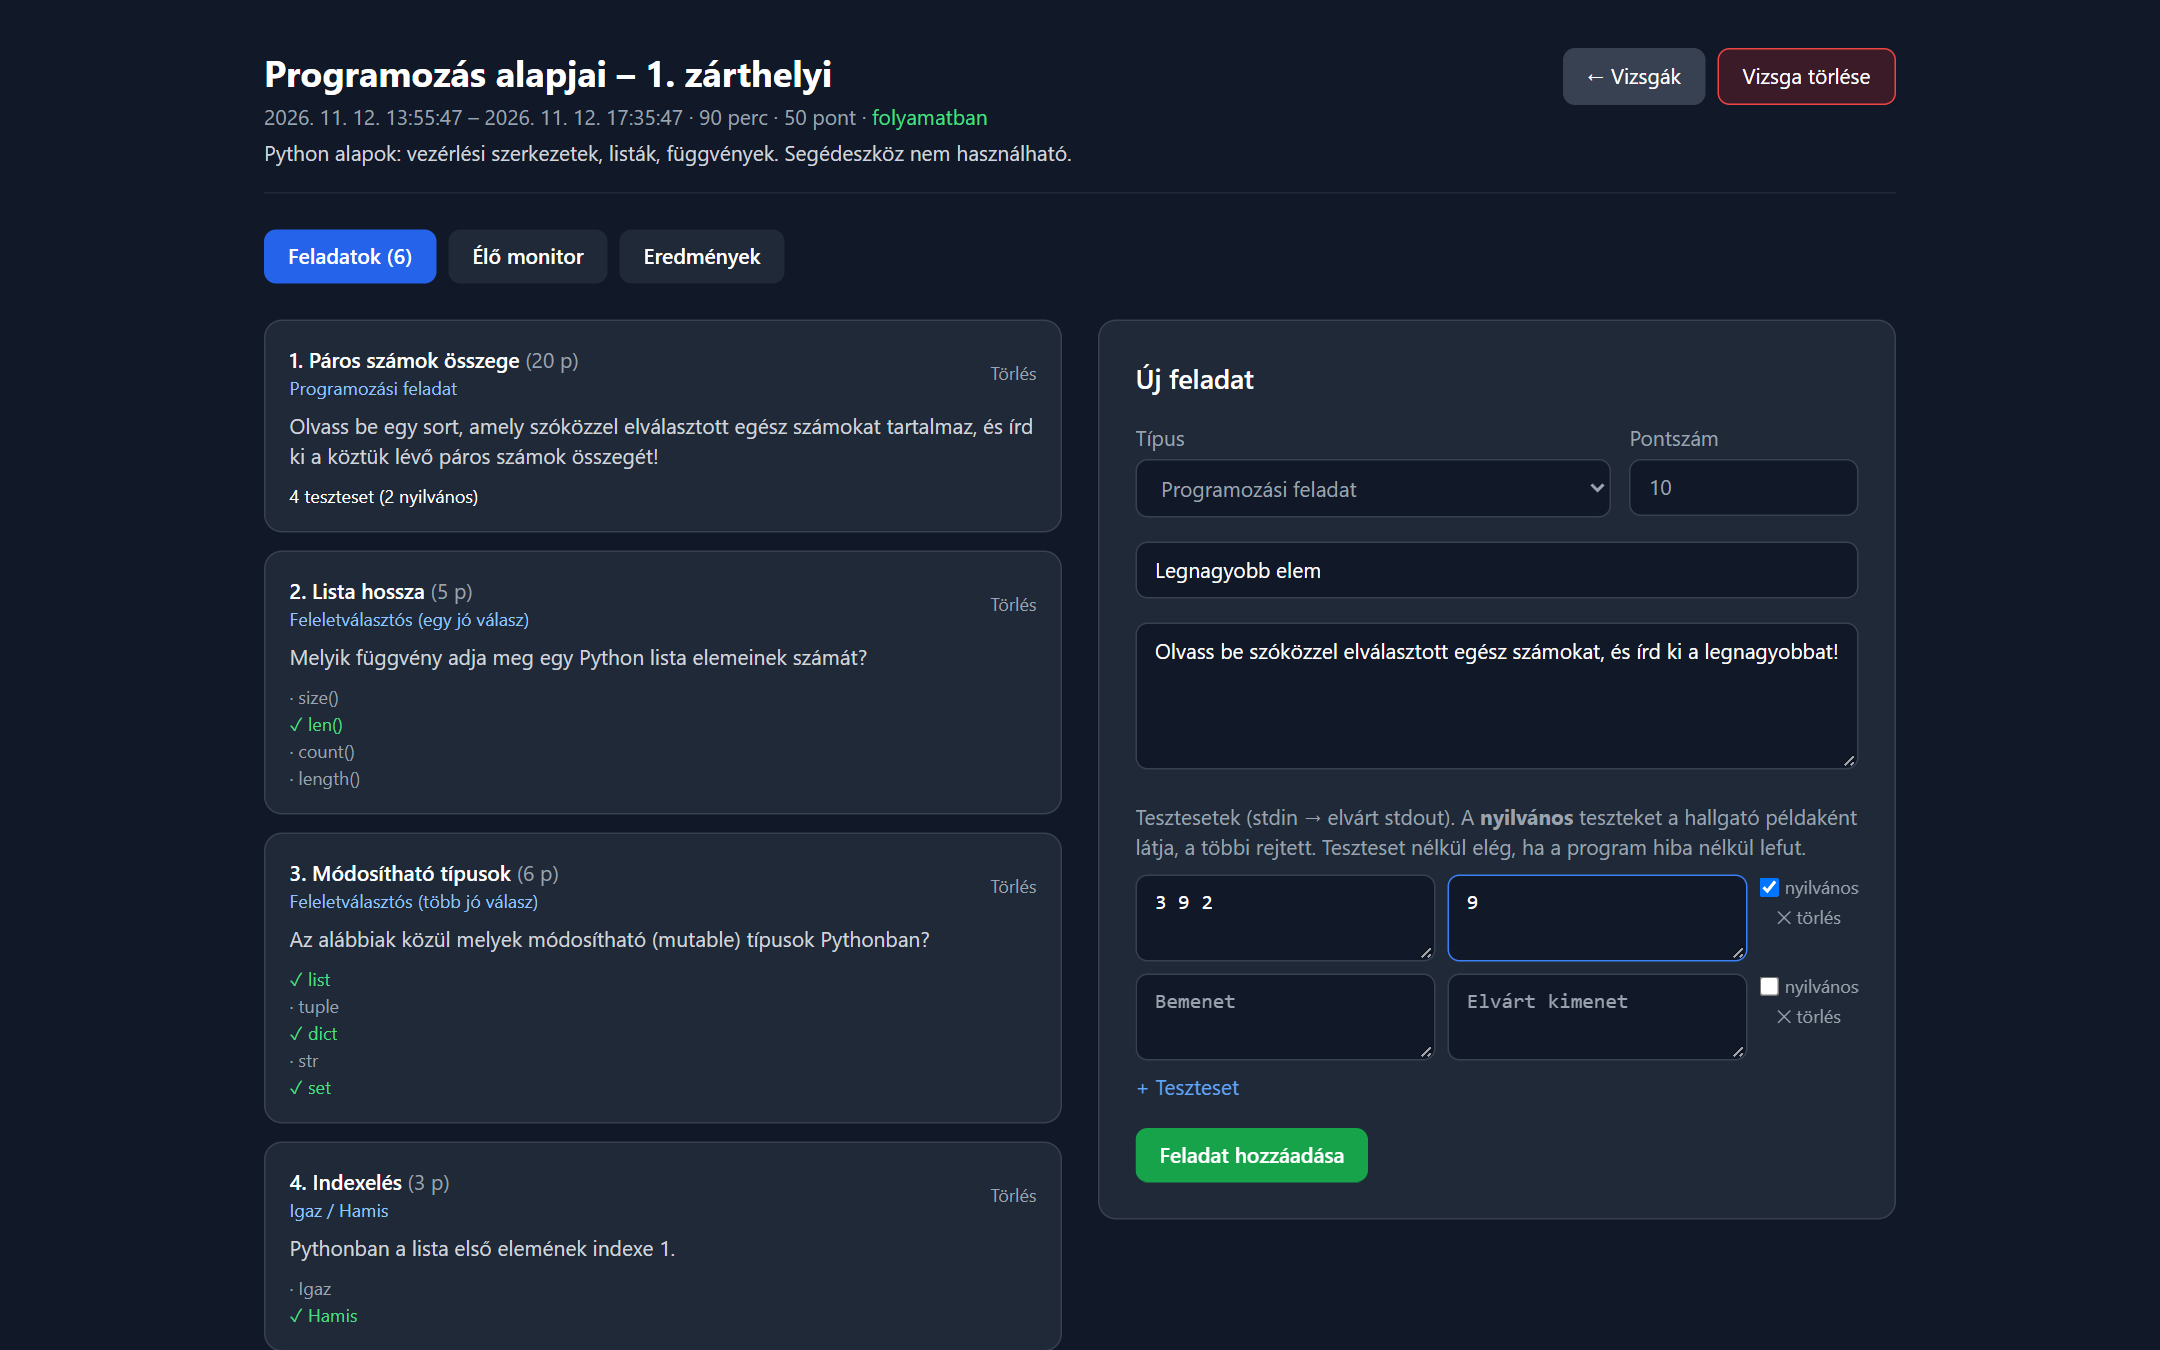
\includegraphics[width=\textwidth]{images/feladatszerkeszto.png}
  \caption{Az oktatói feladatszerkesztő programozási feladat felvétele közben}
  \label{fig:feladatszerkeszto}
\end{figure}

Az élő monitor (\mref{fig:elo_monitor}) a vizsgázókat kártyákon jeleníti meg. A kártya jelzi, hogy
a hallgató éppen dolgozik vagy már beadta a dolgozatát, valamint a figyelmeztetések számát, az
utolsó esemény típusát és időpontját. Ha egy hallgatóhoz legalább egy figyelmeztetés tartozik,
a kártyája piros keretet kap, így az oktató első ránézésre látja, kire kell figyelnie.

\begin{figure}[H]
  \centering
  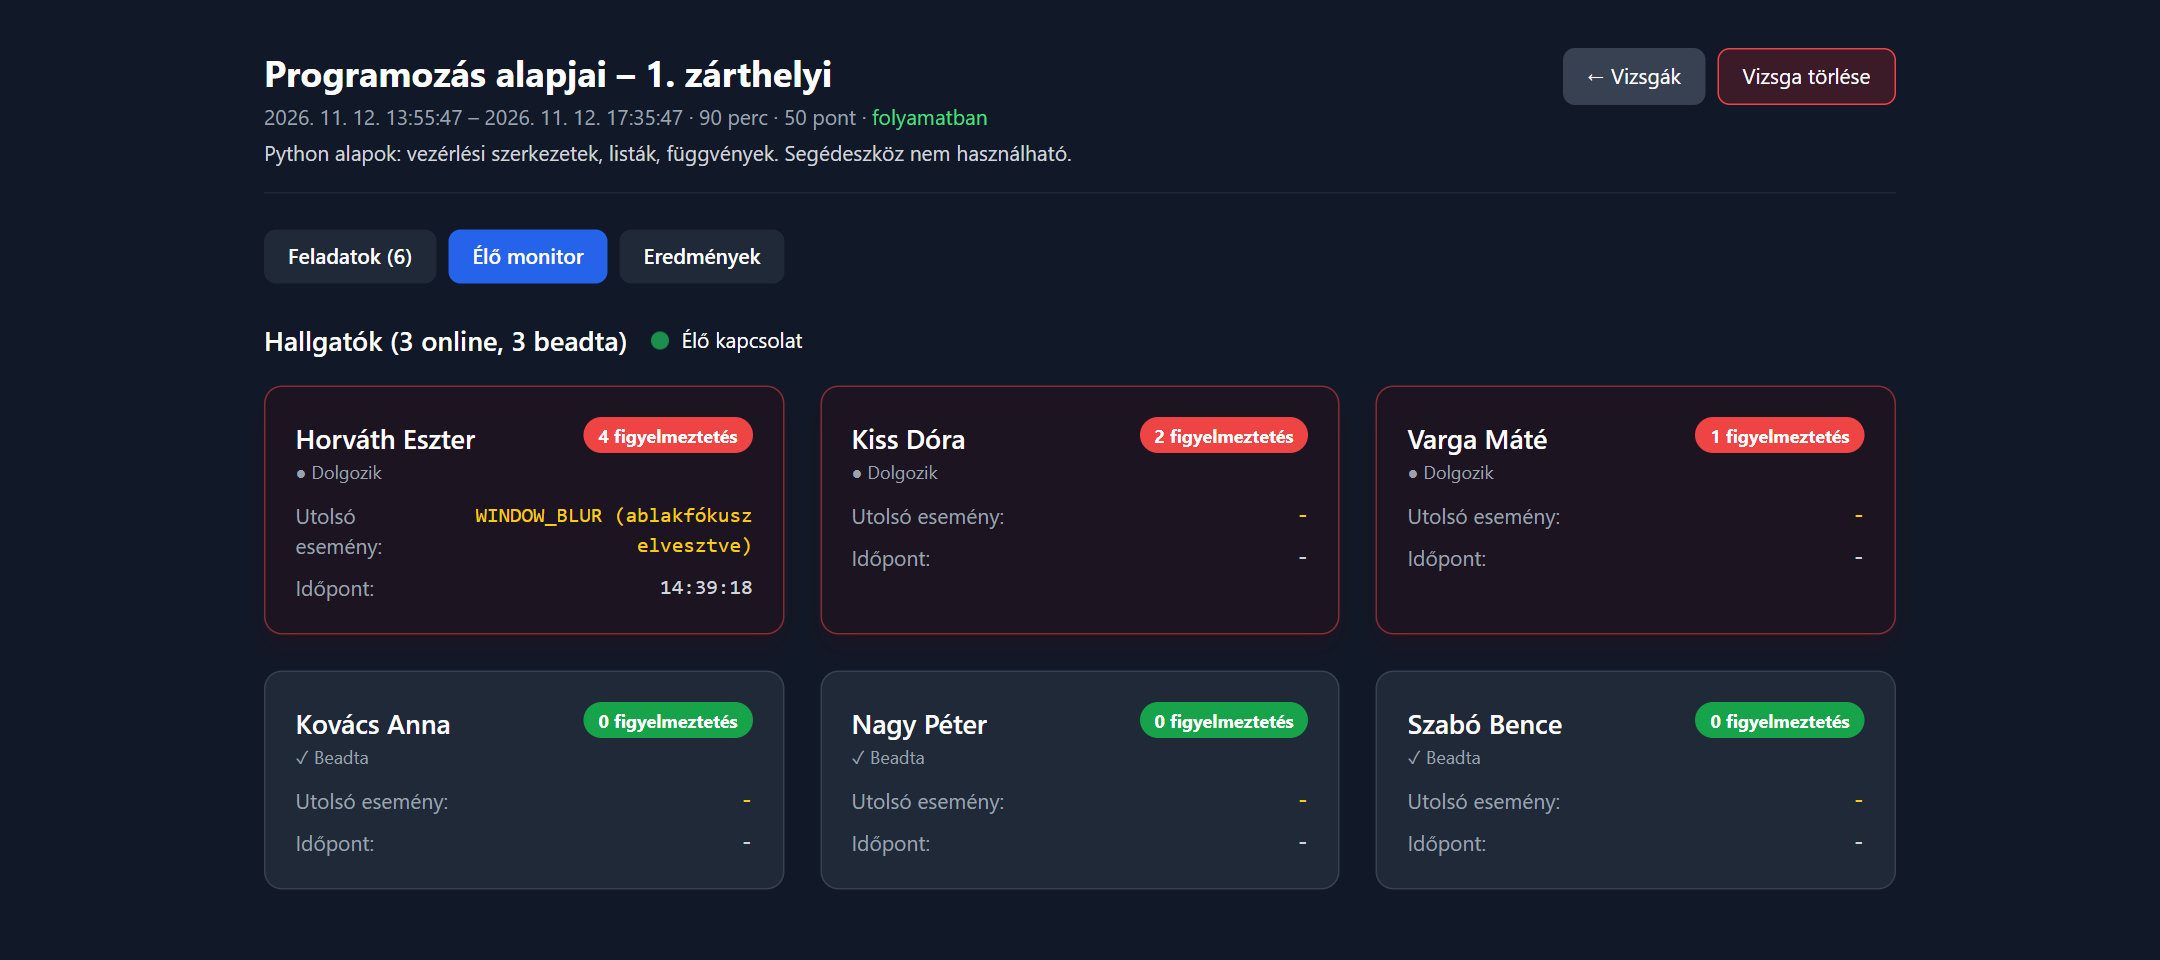
\includegraphics[width=\textwidth]{images/elo_monitor.png}
  \caption{Az élő monitor egy folyamatban lévő vizsga alatt}
  \label{fig:elo_monitor}
\end{figure}

Az eredmények fülön egy hallgató sorát lenyitva feladatonként láthatók a válaszok
(\mref{fig:eredmenyek_reszletes}). Programozási feladatnál a beküldött kód alatt a kódértékelés
részletei is megtekinthetők: az ábrán a hallgató programja a négy tesztesetből hármat teljesített,
ezért 15 pontot kapott a 20-ból. A pontszám alatti mezőkben az oktató felülírhatja az automatikus
pontot, és szöveges visszajelzést írhat.

\begin{figure}[H]
  \centering
  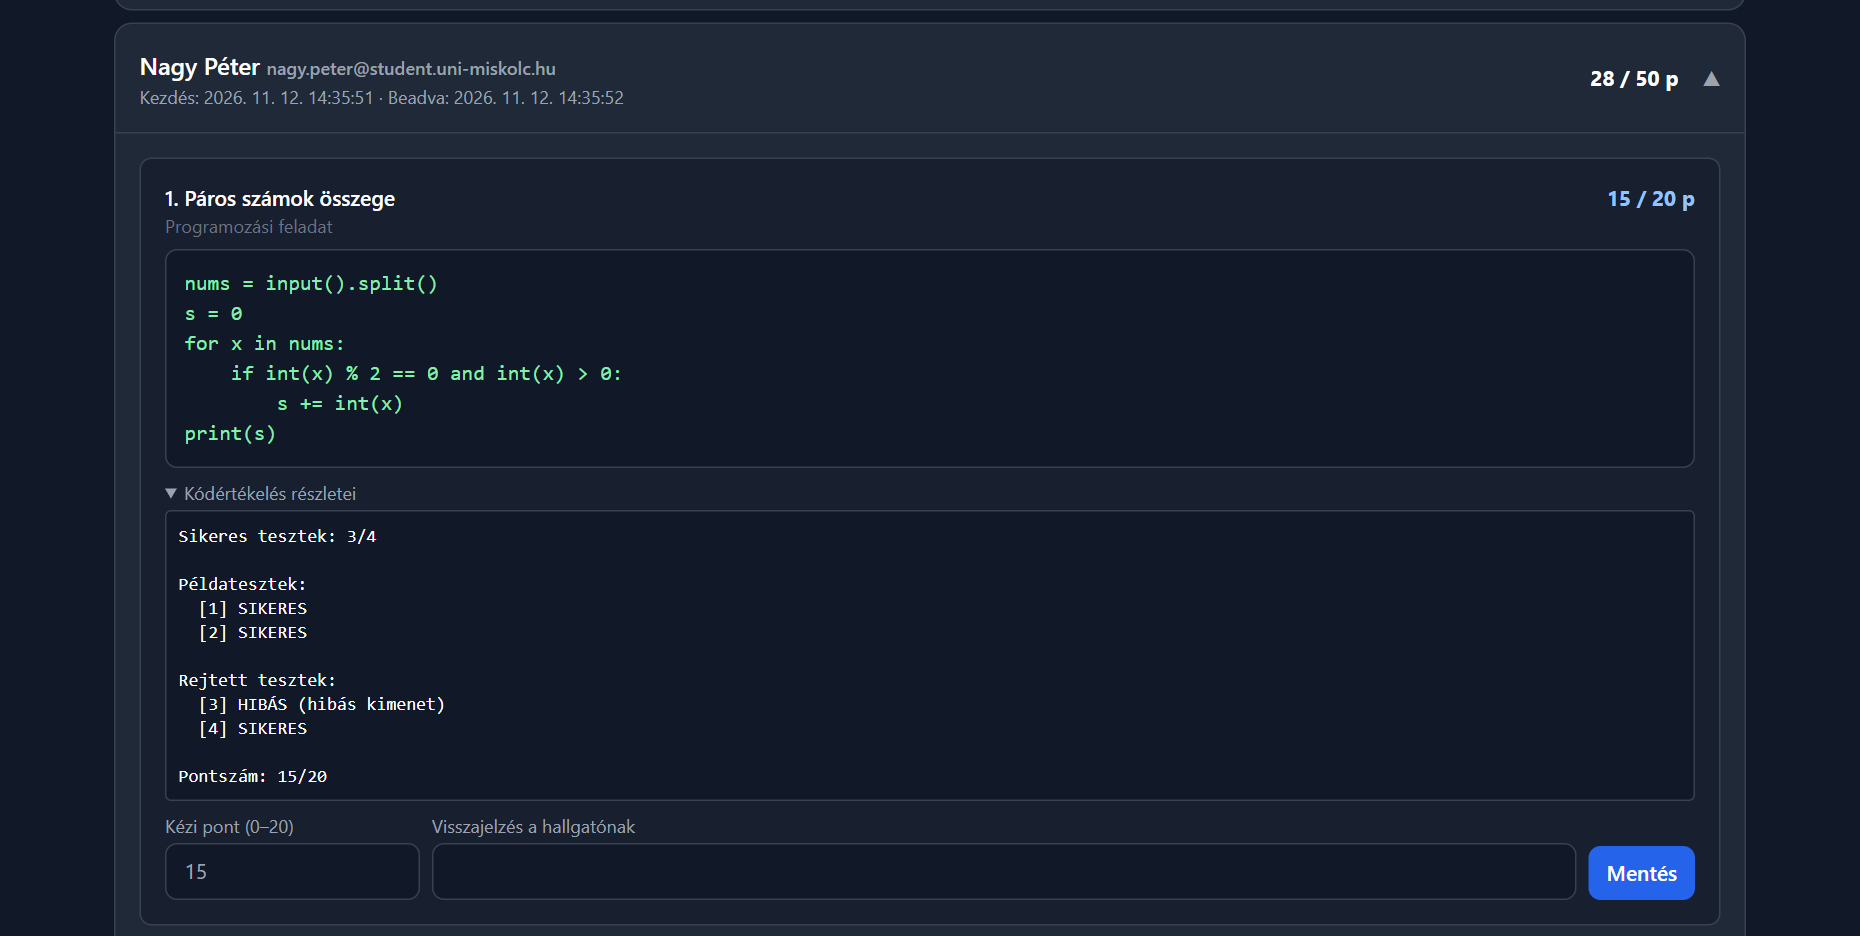
\includegraphics[width=\textwidth]{images/eredmenyek_reszletes.png}
  \caption{Egy hallgató programozási feladatra adott válasza az eredmények fülön}
  \label{fig:eredmenyek_reszletes}
\end{figure}

%!TEX root = ../dolgozat.tex
\chapter{Tesztelés}
\label{ch:teszteles}

Ebben a fejezetben a rendszer tesztelését és a tesztek eredményeit mutatom be. A tesztelés célja
kettős volt: egyrészt annak ellenőrzése, hogy a rendszer megfelel-e \aref{sec:kovetelmenyek}.
szakaszban megfogalmazott funkcionális követelményeknek, másrészt annak igazolása, hogy
\aref{sec:biztonsagi_terv}. szakaszban tervezett védelmek a gyakorlatban is működnek. A fejezet
végén a rendszer használatát is bemutatom.

\section{A tesztelés módszere és környezete}

Sommerville felosztását követve a tesztelés több szinten történhet: a fejlesztői tesztelés az
egyes komponenseket, a rendszertesztelés az összeépített rendszert, az elfogadási tesztelés
pedig a felhasználó szempontjából vizsgálja a szoftvert \cite{sommerville2016software}. Munkám
során a hangsúlyt a rendszertesztelésre helyeztem: a teszteket a kész alkalmazáson, annak
külső interfészein (a REST API-n és a Socket.IO kapcsolaton) keresztül végeztem, így azok
ugyanazt a viselkedést ellenőrzik, amelyet a valódi kliens is tapasztal. A teszteket Python
szkriptekben automatizáltam, így azok bármikor, például egy módosítás után, megismételhetők.

A tesztekhez a következő környezetet használtam: Windows 11 operációs rendszer, Python 3.12.10,
Docker Desktop (Docker Engine 29.9.3), a sandboxban \texttt{python:3.11-slim} image (Python
3.11.18). A funkcionális és a felügyeleti teszteknél minden futtatás egy ideiglenes, üres SQLite
adatbázist használt, így a tesztek egymástól és a fejlesztési adatbázistól függetlenek voltak. Ezt
az teszi lehetővé, hogy a szerveroldal az SQLAlchemy révén adatbázis-független (lásd
\aref{sec:technologiak}. szakaszt), az éles PostgreSQL adatbázissal végzett tesztelés azonban a
jövőben ajánlott kiegészítés.

\section{Funkcionális tesztelés}
\label{sec:funkcionalis_teszt}

A funkcionális teszteket a FastAPI tesztkliensével végeztem, amely valódi HTTP-kéréseket küld az
alkalmazásnak, de nem igényel futó szervert. A tesztszkript először létrehoz két oktatói és két
hallgatói fiókot, majd egy vizsgát különböző típusú feladatokkal, végül végigjátssza a teljes
vizsgafolyamatot. A tesztesetek kiválasztásánál nemcsak a helyes működést ellenőriztem, hanem
szándékosan hibás vagy jogosulatlan kéréseket is küldtem, hiszen egy vizsgarendszernél legalább
olyan fontos, hogy mit \textit{nem} enged meg. A 32 teszteset és az eredményük
\aref{tab:funkcionalis_tesztek}. táblázatban látható.

{\small
\begin{longtable}{@{}lp{9.2cm}p{2.0cm}c@{}}
  \caption{A funkcionális tesztek eredménye}\label{tab:funkcionalis_tesztek}\\
  \toprule
  Azon. & Teszteset & Kapott & Eredmény \\
  \midrule
  \endfirsthead
  \toprule
  Azon. & Teszteset & Kapott & Eredmény \\
  \midrule
  \endhead
  \bottomrule
  \endfoot
  T01 & Oktatói regisztráció hibás meghívókóddal & 400 & sikeres \\
  T02 & Oktatói regisztráció helyes meghívókóddal & oktató & sikeres \\
  T03 & Hallgatói regisztráció (alapértelmezett szerepkör) & hallgató & sikeres \\
  T04 & Regisztráció már foglalt e-mail címmel & 400 & sikeres \\
  T05 & Bejelentkezés hibás jelszóval & 401 & sikeres \\
  T06 & Védett végpont hívása érvénytelen tokennel & 401 & sikeres \\
  T07 & Vizsga létrehozása hallgatói fiókkal & 403 & sikeres \\
  T08 & Vizsga létrehozása hibás időablakkal (a vége a kezdés előtt) & 422 & sikeres \\
  T09 & Feladat létrehozása nem létező helyes válaszra mutató megoldókulccsal & 422 & sikeres \\
  T10 & Feladat hozzáadása más oktató vizsgájához & 403 & sikeres \\
  T11 & Az oktatói (megoldókulcsot tartalmazó) vizsganézet lekérése hallgatóként & 403 & sikeres \\
  T12 & Vizsga kitöltése oktatói fiókkal & 403 & sikeres \\
  T13 & A hallgatónak küldött feladatok nem tartalmaznak megoldókulcsot & nincs benne & sikeres \\
  T14 & A határidő a kezdés + időtartam (60 perc) & 3600 mp & sikeres \\
  T15 & Az ismételt indítás ugyanazt a kitöltést adja vissza & azonos & sikeres \\
  T16 & Egyválasztós feladatnál két válasz mentése & 422 & sikeres \\
  T17 & Nem létező válaszlehetőség mentése & 422 & sikeres \\
  T18 & Mentés egy másik hallgató kitöltésébe & 404 & sikeres \\
  T19 & A pontszám nem látható a beadás előtt & nincs & sikeres \\
  T20 & Egyválasztós feladat helyes válasza teljes pontot ér & 5/5 & sikeres \\
  T21 & Több választós feladat: a 3 helyesből 2 jó és 1 rossz jelölés & 2/6 & sikeres \\
  T22 & Rövid válasz: a ,,\texttt{\ \ 3,14\ }'' válasz elfogadva a ,,\texttt{3.14}'' kulcsra & 3/3 & sikeres \\
  T23 & A kifejtős válasz a beadás után javításra vár & javításra vár & sikeres \\
  T24 & Összpontszám a beadás után ($5+2+2+3$) & 12/26 & sikeres \\
  T25 & Válasz módosítása a beadás után & 409 & sikeres \\
  T26 & Kézi pontozás a feladat maximumánál több ponttal & 422 & sikeres \\
  T27 & Kézi pontozás egy másik oktató vizsgájában & 403 & sikeres \\
  T28 & A kézi pontozás után a hallgató látja a pontot és a visszajelzést & 20/26 & sikeres \\
  T29 & CSV export: UTF-8 bájtsorrend-jelző és pontosvessző elválasztó & megfelelő & sikeres \\
  T30 & Mentés a határidő és a türelmi idő lejárta után & 409 & sikeres \\
  T31 & A lejárt kitöltés automatikus lezárása; a korábban mentett válasz pontot ér & lezárva, 5 p & sikeres \\
  T32 & Vizsga indítása a kezdési időpont előtt & 403 & sikeres \\
\end{longtable}
}

Mind a 32 teszteset az elvárt eredményt adta. Külön kiemelném a T21-es és a T31-es esetet. A T21
\mref{sec:pontozas}ban ismertetett részpontozási képletet ellenőrzi: a hat pontos feladatnál a
hallgató a három helyes válaszból kettőt, valamint egy hibás választ jelölt meg, így a pontszáma
$\max(0, (2-1)/3) \cdot 6 = 2$ pont. A T31-es teszthez a kitöltés határidejét közvetlenül az
adatbázisban állítottam a múltba, ezzel szimulálva azt a helyzetet, amikor a hallgató a vizsga
közben bezárja a böngészőt, és többé nem tér vissza. A rendszer a következő lekérdezéskor
lezárta a kitöltést, és a korábban automatikusan elmentett választ értékelte, vagyis a hallgató
munkája nem veszett el.

\section{A sandbox biztonsági tesztelése}
\label{sec:sandbox_teszt}

A kódfuttatás biztonságát úgy ellenőriztem, hogy szándékosan ártó programokat futtattam a
valódi Docker-sandboxban, ugyanazon a függvényen keresztül, amelyet a rendszer a hallgatói
megoldások értékelésére használ. Minden tesztprogram egy-egy fenyegetést valósít meg
\aref{sec:sandbox_elmelet}. szakaszban felsoroltak közül. Az eredményeket és az egyes futtatások
teljes idejét (a konténer indításával és törlésével együtt) \aref{tab:sandbox_tesztek}. táblázat
tartalmazza.

{\small
\begin{longtable}{@{}l>{\raggedright\arraybackslash}p{3.9cm}>{\raggedright\arraybackslash}p{6.2cm}rc@{}}
  \caption{A sandbox biztonsági tesztjeinek eredménye}\label{tab:sandbox_tesztek}\\
  \toprule
  Azon. & Támadás & A rendszer reakciója & Idő & Eredmény \\
  \midrule
  \endfirsthead
  \toprule
  Azon. & Támadás & A rendszer reakciója & Idő & Eredmény \\
  \midrule
  \endhead
  \bottomrule
  \endfoot
  B01 & Végtelen ciklus & időtúllépés az 5 mp-es korlátnál & 5,52 s & védett \\
  B02 & Fork bomb (folyamatok indítása ciklusban) & a 64-es folyamatkorlát miatt az \texttt{os.fork} hibát jelez (\textit{Resource temporarily unavailable}) & 0,66 s & védett \\
  B03 & 1 GB memória lefoglalása & a kernel a folyamatot leállítja (SIGKILL, kilépési kód $-9$) & 1,31 s & védett \\
  B04 & Hálózati kapcsolat egy külső címre & \textit{Network is unreachable} & 0,63 s & védett \\
  B05 & Fájl írása az \texttt{/etc} könyvtárba & \textit{Read-only file system} & 0,46 s & védett \\
  B06 & Végtelen mennyiségű kimenet & a kimenet 64 KB-nál csonkolva, majd időtúllépés & 5,44 s & védett \\
  B07 & A vezérlő környezeti változóinak (kód, tesztek) kiolvasása & a hallgató folyamata nem látja őket & 0,45 s & védett \\
  B08 & Az eredményjelölő (\texttt{\_\_RESULTS\_\_}) kiírása a kimenetre & eredetileg az értékelés rendszerhibával leállt; a javítás után a program kimenete közönséges szövegként jelenik meg (lásd a szöveget) & 0,48 s & javítva \\
  B09 & A vezérlőfolyamat leállítása (\texttt{kill 1}) & \textit{Operation not permitted} & 0,55 s & védett \\
  B10 & A futtató felhasználó lekérdezése & UID és GID: 65534 (\texttt{nobody}) & 0,49 s & megfelelő \\
\end{longtable}
}

A tíz tesztből kilenc igazolta a tervezett védelem működését. A végtelen ciklust és a végtelen
kimenetet az időkorlát állította meg, a fork bombát a folyamatszám-korlát, a memóriafoglalást a
konténer memóriakorlátja. A hálózat és a fájlrendszer elérése nem volt lehetséges, a hallgató
programja pedig nem férhetett hozzá a vezérlő adataihoz, és nem állíthatta le azt. A B03-as
tesztnél érdemes megjegyezni, hogy a memóriakorlát túllépésekor a program nem kap Python
kivételt, hanem a kernel azonnal leállítja; a rendszer ezt futási hibaként értékeli.

A B08-as teszt azonban hibát tárt fel. A vezérlőprogram az eredményeket a kimenete végére, egy
\texttt{\_\_RESULTS\_\_} jelölő után írta ki JSON formátumban, a szerver pedig a jelölő
\textit{utolsó} előfordulását kereste meg a konténer kimenetében. A hallgató programjának kimenete
azonban maga is bekerül ebbe a JSON-ba, így ha a program kiírta a jelölő szövegét, a szerver a
JSON belsejében találta meg az utolsó előfordulást, a feldolgozás meghiúsult, és az értékelés
,,Rendszerhiba'' üzenettel állt le. A hiba a pontszám meghamisítására nem adott lehetőséget, mert a
hallgató kimenete a JSON-ban idézőjelek között, megfelelően kódolva szerepel, így abból érvényes
eredménylista nem állítható elő; a következménye az volt, hogy az érintett válasz pontozatlan maradt.

A hibát két lépésben javítottam. Mivel a vezérlőprogram a jelölő előtt semmit nem ír ki, és a
hallgató kimenete csak a jelölő utáni JSON-ban szerepelhet, a szerver most a jelölő
\textit{első} előfordulását keresi meg. Emellett a jelölő már nem rögzített szöveg: a szerver
minden kiértékeléshez egy véletlenszerű, 128 bites azonosítót tartalmazó jelölőt
(\texttt{\_\_RESULTS\_<véletlen hexa>\_\_}) generál, és azt csak a vezérlőprogram környezeti
változójában adja át. A hallgató programjának környezetébe ez nem kerül át, és a vezérlő
folyamat környezetét (\texttt{/proc/1/environ}) sem olvashatja, így a jelölőt nem ismerheti.
A javítás után megismételt tesztben a jelölő szövegét kiíró program kimenete közönséges
szövegként jelent meg az eredményben, a \texttt{\_\_RESULTS\_\_} szöveget elvárt kimenetként
megadó feladatot pedig a rendszer helyesen, teljes pontszámmal értékelte.

\section{Teljesítmény}
\label{sec:teljesitmeny}

A programozási feladatok értékelésének sebességét két szempontból vizsgáltam. A pontozás
helyességét egy két tesztesetből (egy nyilvános és egy rejtett) álló, tízpontos feladaton
ellenőriztem: a helyes megoldás 10, a hibás 0 pontot kapott, és a hibás megoldás visszajelzésében
a rejtett teszteset bemenete nem jelent meg. Ezután megmértem, hogyan függ az értékelés ideje a
tesztesetek számától (\mref{tab:teljesitmeny}).

\begin{table}[H]
  \centering
  \caption{Egy kiértékelés átlagos ideje a tesztesetek számának függvényében (3 futás átlaga)}
  \label{tab:teljesitmeny}
  \begin{tabular}{@{}rr@{}}
    \toprule
    Tesztesetek száma & Átlagos idő \\
    \midrule
    1  & 0,44 s \\
    10 & 0,76 s \\
    20 & 1,04 s \\
    \bottomrule
  \end{tabular}
\end{table}

Az eredmények igazolják \mref{sec:sandbox}ban leírt tervezési döntést. Egy kiértékelés idejének
nagyobb részét a konténer indítása és törlése teszi ki (kb. 0,4 másodperc), egy-egy további
teszteset pedig csak körülbelül 30 milliszekundummal növeli az időt. Ha minden tesztesethez
külön konténer indulna, egy 20 tesztesetből álló feladat értékelése ennek alapján
nagyságrendileg 8--9 másodpercig tartana az egy konténerrel mért egy másodperc helyett. A mért
idők bőven megfelelnek a követelményeknek, hiszen a hallgató a beküldés után egy másodpercen belül
megkapja az eredményt. Megjegyzendő, hogy a mérés egyetlen felhasználóval, fejlesztői gépen
készült; terheléses tesztelést, vagyis sok egyidejű beküldés vizsgálatát nem végeztem.

\section{A valós idejű felügyelet tesztelése}
\label{sec:felugyelet_teszt}

A felügyelet szerveroldali működését egy futó szerverrel és Python nyelvű Socket.IO kliensekkel
teszteltem, amelyek a hallgatói és az oktatói klienst szimulálták. Az eredményeket
\aref{tab:socket_tesztek}. táblázat tartalmazza.

{\small
\begin{longtable}{@{}lp{8.6cm}p{2.6cm}c@{}}
  \caption{A valós idejű felügyelet tesztjeinek eredménye}\label{tab:socket_tesztek}\\
  \toprule
  Azon. & Teszteset & Kapott & Eredmény \\
  \midrule
  \endfirsthead
  \toprule
  Azon. & Teszteset & Kapott & Eredmény \\
  \midrule
  \endhead
  \bottomrule
  \endfoot
  S01 & Csatlakozás token nélkül & elutasítva & sikeres \\
  S02 & Csatlakozás érvénytelen tokennel & elutasítva & sikeres \\
  S03 & Egy másik oktató belépése a vizsga szobájába & elutasítva & sikeres \\
  S04 & Hallgató belépése folyamatban lévő kitöltés nélkül & elutasítva & sikeres \\
  S05 & Az oktató belépéskor pillanatképet kap a kitöltésekről & megkapta & sikeres \\
  S06 & Az oktató értesítést kap a hallgató belépéséről & megkapta & sikeres \\
  S07 & 10 ablakelhagyás jelzése az oktatónak & 10 riasztás & sikeres \\
  S08 & A szabálysértések száma az adatbázisban is megjelenik & 10 & sikeres \\
  S09 & Beadáskor az oktató értesítést kap & megkapta & sikeres \\
  S10 & A beadás után küldött jelzés figyelmen kívül marad & nincs riasztás & sikeres \\
\end{longtable}
}

Mind a tíz teszteset sikeres volt. Az S07-es tesztben azt is megmértem, mennyi idő telik el a
hallgatói kliens jelzésének elküldése és a riasztás oktatói klienshez érkezése között: tíz mérés
alapján az átlag 8,9 ms volt (legkisebb 8,2 ms, legnagyobb 11,1 ms). A tesztkliens a WebSocket
helyett HTTP hosszú lekérdezéssel kommunikált, a mérés pedig egyetlen gépen, helyi hálózaton
történt, így valós hálózati körülmények között a hálózati késleltetés is hozzáadódik; a riasztás
az oktató számára ennek ellenére gyakorlatilag azonnalinak tekinthető.

A kliensoldali érzékelést, vagyis azt, hogy a böngésző valóban jelzi-e az ablak elhagyását, csak
valódi böngészőben lehet ellenőrizni. A tesztet Windows 11 operációs rendszeren, a Google Chrome
157-es verziójával végeztem. A hallgatói vizsgaoldalt egy önálló Chrome-ablakban nyitottam meg,
és a műveleteket valódi billentyűparancsokkal (\texttt{Ctrl+T}, \texttt{Ctrl+W}, \texttt{Ctrl+L},
\texttt{F5}), illetve az ablak kis méretre állításával és egy másik alkalmazás előtérbe hozásával
hajtottam végre. Minden lépés után összevetettem a hallgatói fejlécben látható ablakváltás-számlálót,
az oktatói oldalon megjelenő értéket és az oldalon kiváltott böngészőesemények sorrendjét. Az
eredményeket \aref{tab:bongeszo_tesztek}. táblázat foglalja össze.

{\small
\begin{longtable}{@{}l>{\raggedright\arraybackslash}p{4.2cm}>{\raggedright\arraybackslash}p{6.4cm}c@{}}
  \caption{A böngészőoldali felügyelet tesztjeinek eredménye}\label{tab:bongeszo_tesztek}\\
  \toprule
  Azon. & Művelet & Kiváltott események & Figyelm. \\
  \midrule
  \endfirsthead
  \toprule
  Azon. & Művelet & Kiváltott események & Figyelm. \\
  \midrule
  \endhead
  \bottomrule
  \endfoot
  K01 & Új lap megnyitása, majd visszatérés a vizsgafülre & \texttt{blur}, \texttt{visibilitychange} (\textit{hidden}), \texttt{visibilitychange} (\textit{visible}), \texttt{focus} & 1 \\
  K02 & Váltás másik alkalmazásra (Alt+Tab) & \texttt{blur} & 1 \\
  K03 & Ablak kis méretre állítása, majd visszaállítása & \texttt{blur}, \texttt{visibilitychange} (\textit{hidden}), \texttt{visibilitychange} (\textit{visible}), \texttt{focus} & 1 \\
  K04 & Az oldal frissítése (F5) & \texttt{pagehide}, \texttt{visibilitychange} (\textit{hidden}) & 0\textsuperscript{*} \\
  K05 & Kattintás a böngésző címsorába & \texttt{blur} & 1 \\
  \multicolumn{4}{@{}l}{\footnotesize\textsuperscript{*}A javítás előtt 1 (lásd a szöveget).}\\
\end{longtable}
}

A fülváltás (K01) és a kis méretre állítás (K03) esetén a böngésző két eseményt is küld az ablak
elhagyásakor: a fókusz elvesztését (\texttt{blur}) és a lap elrejtését (\texttt{visibilitychange}).
A kliens ezeket egyetlen elhagyásnak tekinti, mert az első esemény után egy jelzőt állít be, amelyet
csak az ablak újbóli fókuszba kerülése (\texttt{focus}) töröl; a fülváltás így a tervezettnek
megfelelően egyszer számít. Másik alkalmazásra váltáskor (K02) a lap látható marad, ezért csak a
\texttt{blur} esemény érkezik, ez is egy figyelmeztetést eredményezett. A számláló értéke minden
esetben azonnal megjelent az oktatói monitoron, és megegyezett az adatbázisban tárolt értékkel.

A teszt két olyan esetre is rávilágított, amikor a rendszer a hallgató szándékától függetlenül
jelzett. Az oldal frissítésekor (K04) a böngésző a régi oldal elhagyása előtt elrejtettnek jelöli a
lapot, és a kliens eredetileg ezt is elküldte a szervernek, így minden frissítés egy
figyelmeztetést okozott. A hibát úgy javítottam, hogy a kliens a \texttt{pagehide} eseményre,
vagyis az oldal elhagyásának kezdetére egy jelzőt állít be, és ezután nem küld több figyelmeztetést;
ha a böngésző a vissza gombbal a gyorsítótárból állítja vissza az oldalt (\texttt{pageshow}), a
jelző törlődik. Az oldal elhagyása így sem marad észrevétlen, mert a Socket.IO-kapcsolat ilyenkor
megszakad, és az oktatói monitor a hallgatót kilépettként jelzi. A javítás után megismételt
tesztben három egymást követő frissítés sem okozott figyelmeztetést, a fülváltás és a kis méretre
állítás viszont továbbra is egy-egy figyelmeztetést eredményezett, a frissítés után is. A
számláló értéke a frissítéskor nem nullázódik, mert a kliens a szervertől kapja vissza a tárolt
értéket.

A böngésző címsorába kattintás (K05) szintén elveszi a fókuszt az oldaltól, ezért figyelmeztetésnek
számít. Ezt a böngésző eseményei alapján nem lehet megkülönböztetni attól, amikor a hallgató egy
másik alkalmazásra vált, ezért ezen nem változtattam. Mivel ilyenkor a hallgató valójában nem
hagyta el a vizsgát, az oktatónak a figyelmeztetések számát nem önmagában, hanem a többi
körülménnyel együtt érdemes értékelnie.

\section{Az alkalmazás használata}
\label{sec:hasznalat}

Ebben a szakaszban röviden, a felhasználó szemszögéből mutatom be a rendszer használatát. A
telepítés lépéseit a dolgozat végén található adathordozó-útmutató tartalmazza.

\paragraph{Oktatóként.} Az oktató a regisztrációs űrlapon az ,,Oktatóként regisztrálok''
lehetőséget választva, a meghívókód megadásával hozhat létre fiókot. Bejelentkezés után az oktatói
felületen új vizsgát hozhat létre, megadva a címét, a leírását, a kezdési és záró időpontot,
valamint a kitöltésre szánt időt. A vizsga oldalán három fül található. A \textit{Feladatok} fülön
adhatók hozzá a feladatok; az űrlap a kiválasztott feladattípushoz igazodik, programozási
feladatnál például a tesztesetek bemenete, elvárt kimenete és láthatósága adható meg. Az
\textit{Élő monitor} fülön a vizsga ideje alatt az oktató látja, mely hallgatók vannak éppen
jelen, hányszor hagyták el a vizsgaablakot, és ki adta már be a dolgozatát. Az
\textit{Eredmények} fülön hallgatónként áttekintheti a válaszokat, pontozhatja a kifejtős
feladatokat, felülírhatja az automatikus pontszámot, szöveges visszajelzést írhat, és az
eredményeket CSV fájlba exportálhatja.

\paragraph{Hallgatóként.} A hallgató a regisztráció és a bejelentkezés után a műszerfalon látja az
elérhető vizsgákat, a vizsgák időpontját, a feladatok számát és az elérhető pontszámot. A vizsga
elindítása után a képernyő tetején rögzített fejléc mutatja a hátralévő időt, a felügyeleti
kapcsolat állapotát (,,Felügyelet aktív'') és az eddigi ablakváltások számát; alatta egy
gombsorban választhatók ki a feladatok, ahol pipa jelzi a már megválaszoltakat. A válaszok
gépelés közben automatikusan mentődnek. Programozási feladatnál a hallgató a kódját a
,,Próbafuttatás'' gombbal kipróbálhatja a nyilvános példatesztekkel vagy saját bemenettel, a
,,Beküldés \& értékelés'' gombbal pedig az összes tesztesettel értékeltetheti, és azonnal látja,
hány teszt volt sikeres. A ,,Vizsga beadása'' gomb megnyomása után -- illetve az idő lejártakor
automatikusan -- a vizsga lezárul, és a hallgató megtekintheti az eredményét.

Az oktatói felület kezdőoldalát \aref{fig:oktatoi_muszerfal}. ábra mutatja: bal oldalon az oktató
vizsgái láthatók az állapotukkal (,,Hamarosan'', ,,Folyamatban''), jobb oldalon az új vizsga
létrehozására szolgáló űrlap. A feladatszerkesztőt, az élő monitort és az eredmények részletes
nézetét \aref{sec:felulet}. szakaszban mutattam be
(\mref{fig:feladatszerkeszto}, \mref{fig:elo_monitor}, \mref{fig:eredmenyek_reszletes}).

\begin{figure}[H]
  \centering
  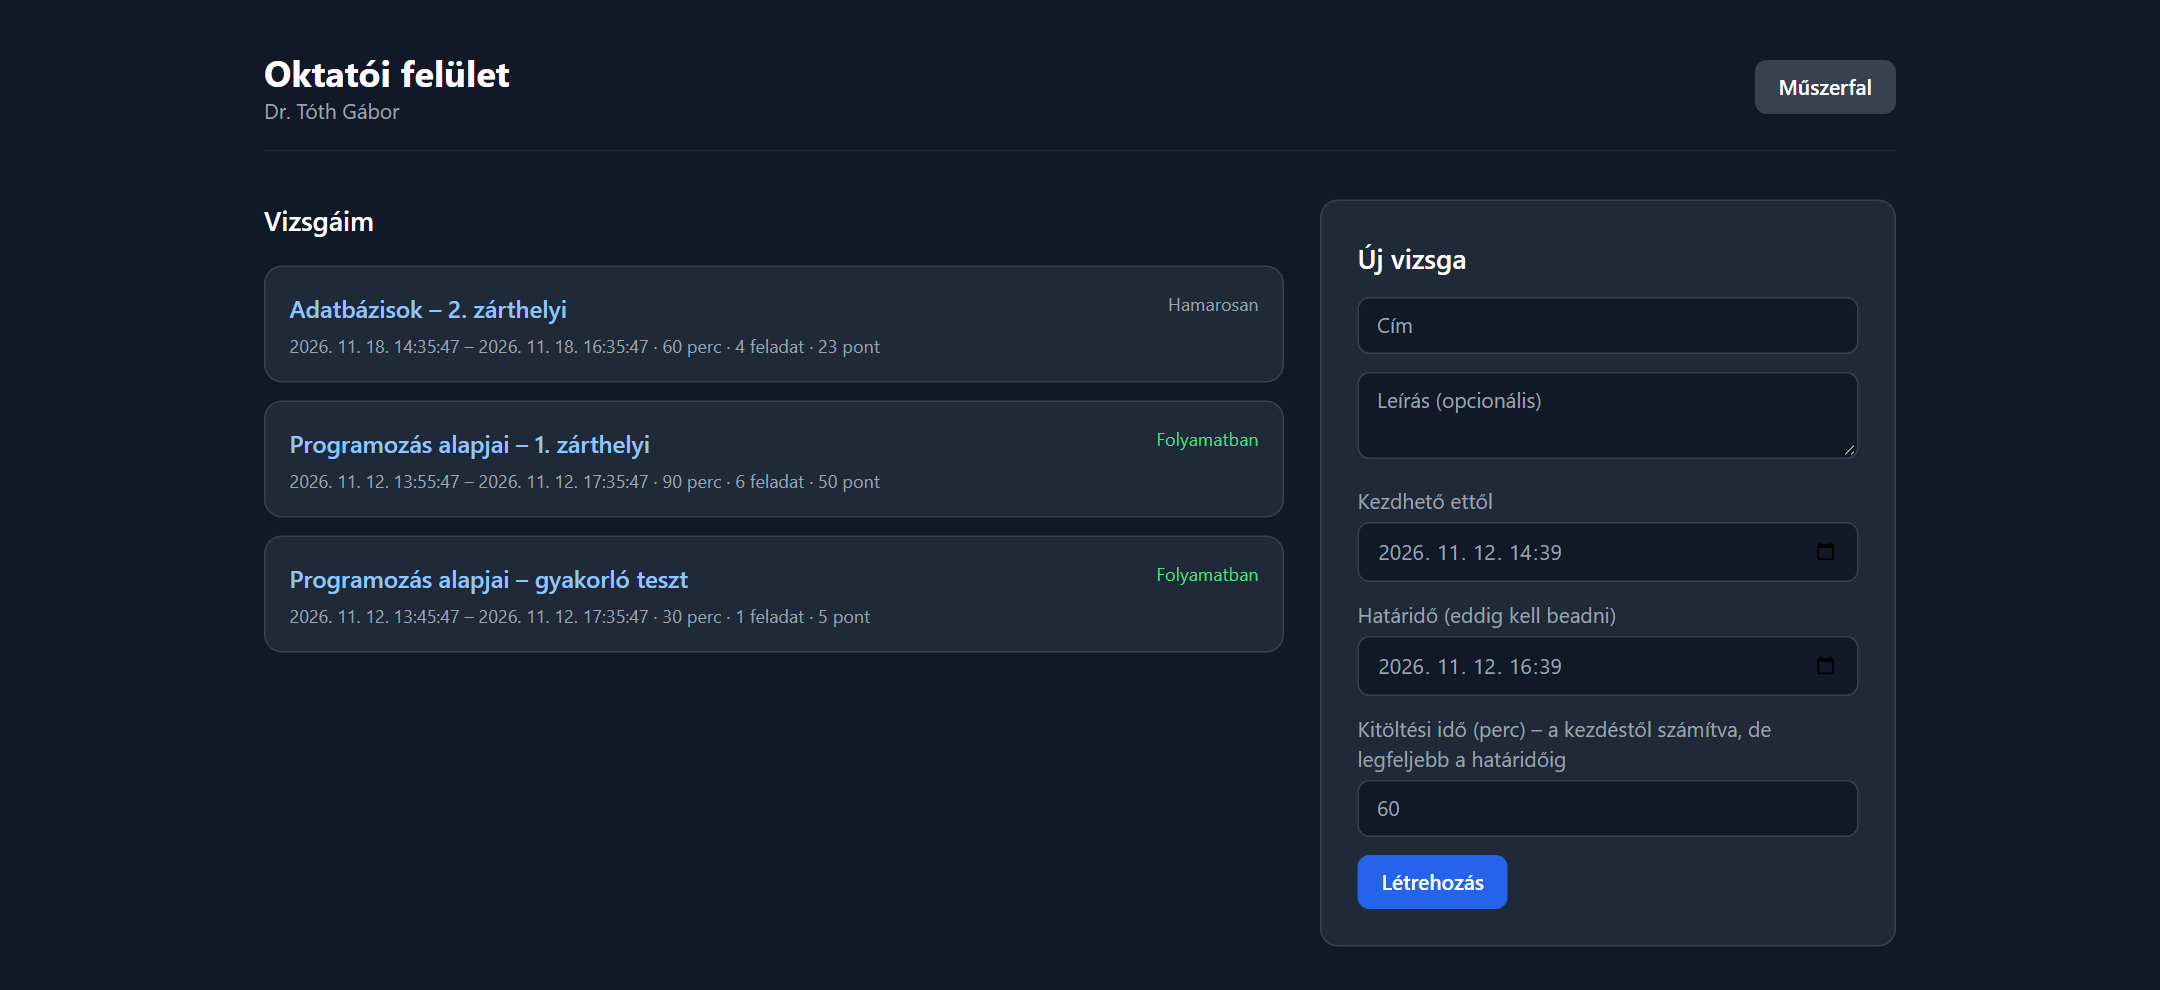
\includegraphics[width=\textwidth]{images/oktatoi_muszerfal.png}
  \caption{Az oktatói felület a vizsgák listájával és az új vizsga űrlapjával}
  \label{fig:oktatoi_muszerfal}
\end{figure}

Az eredmények fül összesítő nézetében (\mref{fig:eredmenyek}) a hallgatók egy-egy sorban
szerepelnek a kezdés és a beadás időpontjával, az ablakváltások számával és a pontszámukkal. A
lista felett a kitöltések száma, az átlagpontszám és a még javításra váró válaszok száma látható,
itt érhető el a CSV export és az újraértékelés is.

\begin{figure}[H]
  \centering
  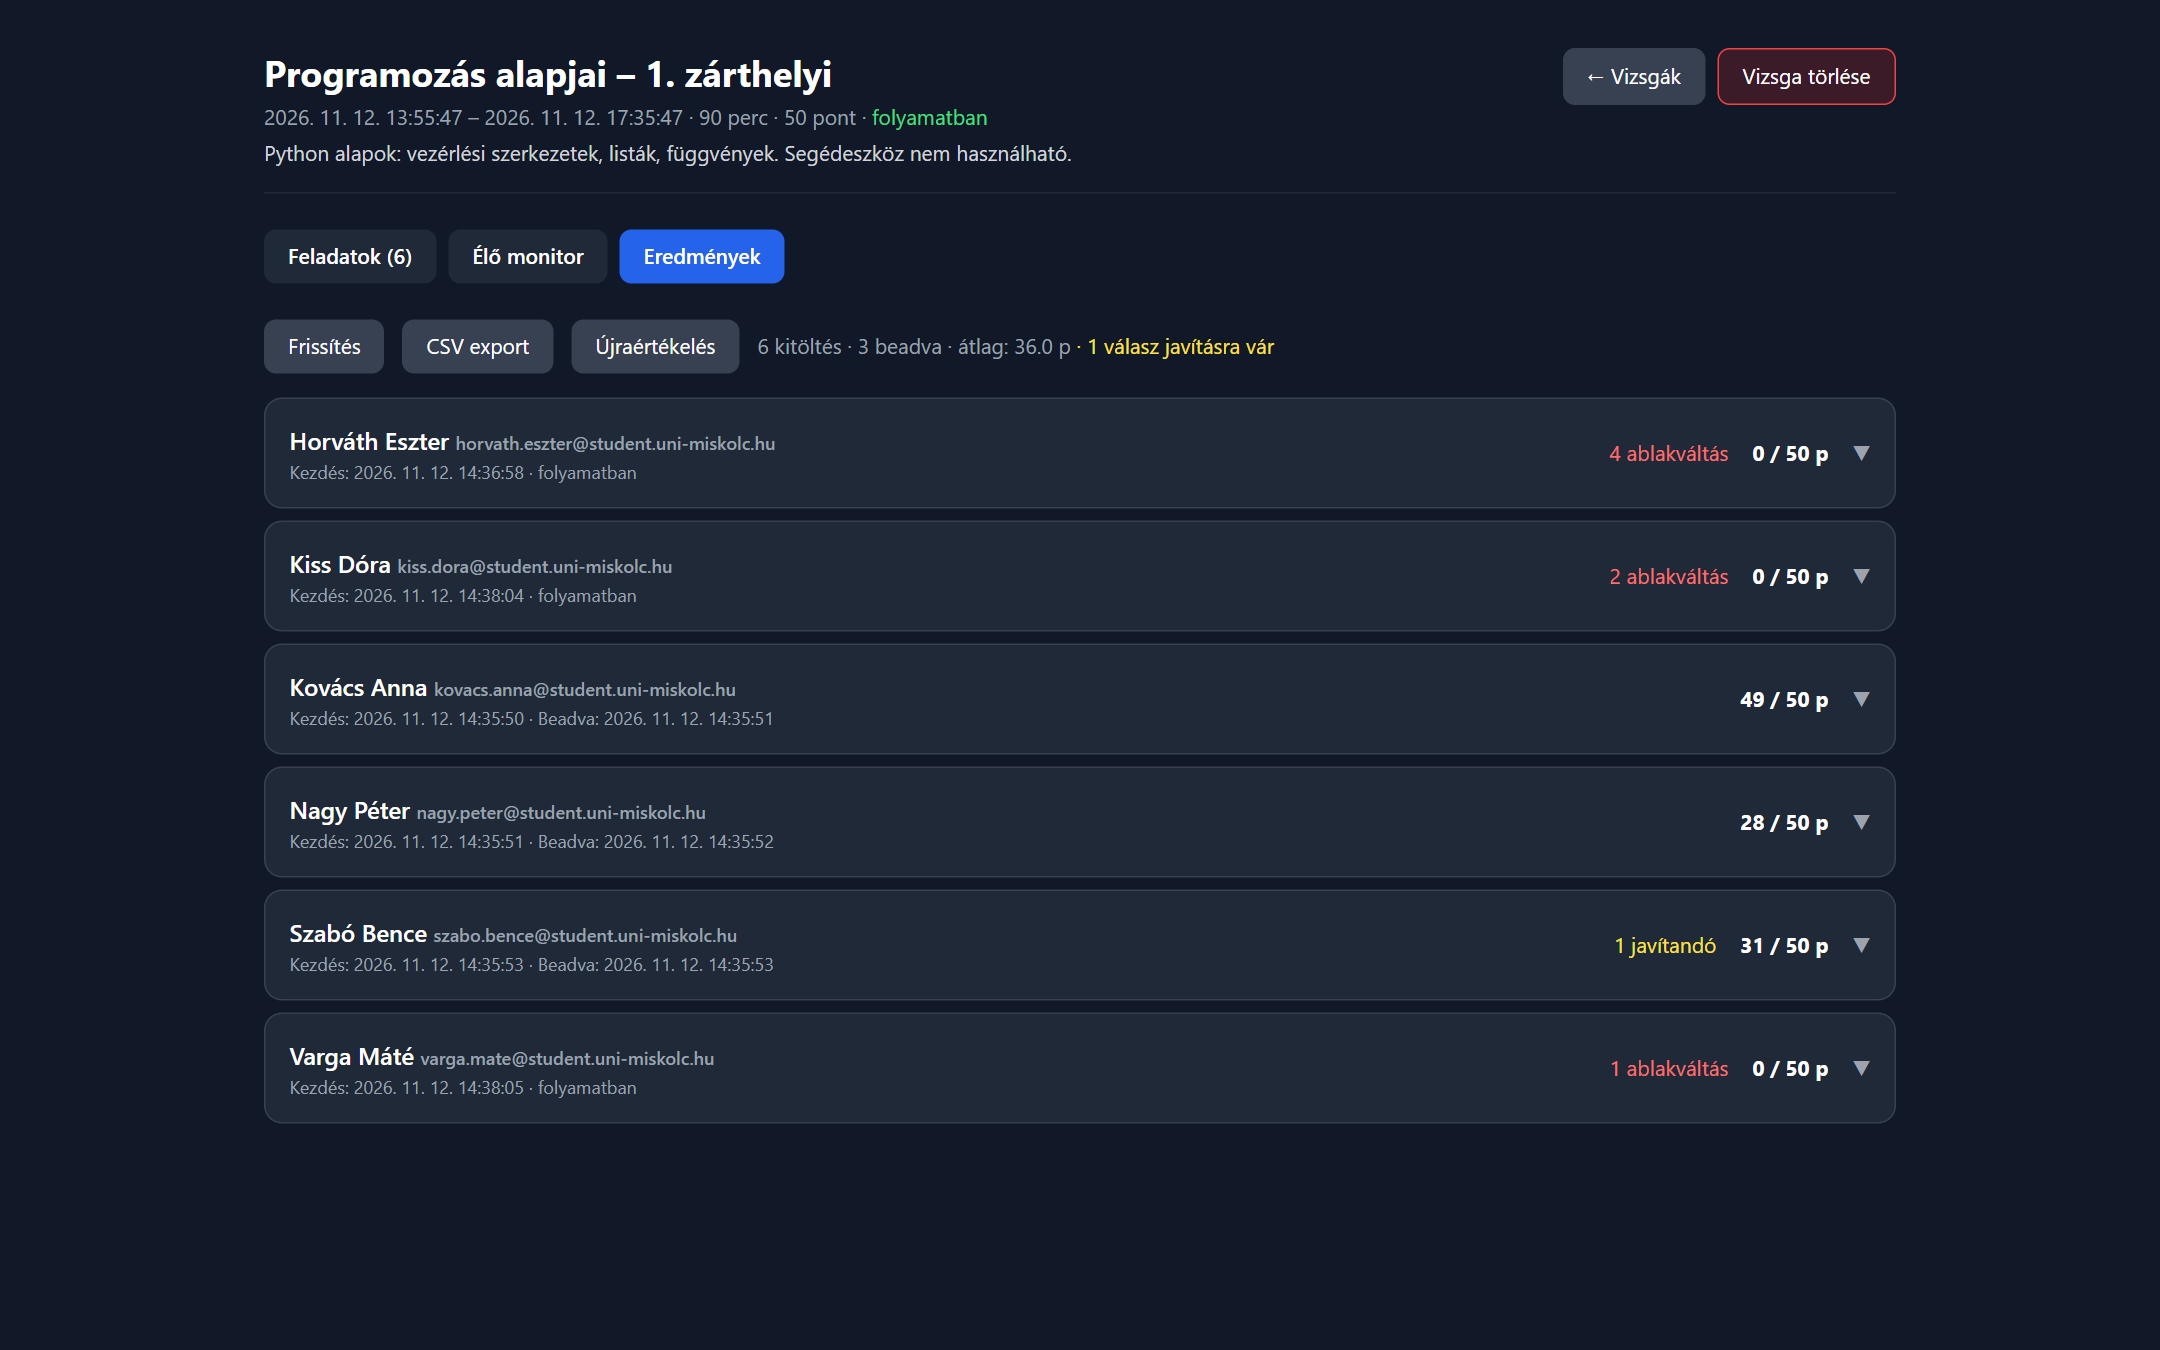
\includegraphics[width=\textwidth]{images/eredmenyek.png}
  \caption{Az eredmények fül összesítő nézete}
  \label{fig:eredmenyek}
\end{figure}

A hallgatói műszerfalat \aref{fig:hallgatoi_muszerfal}. ábra mutatja. Minden vizsga külön kártyán
jelenik meg; a kártya alján lévő gomb az állapottól függően a vizsga indítására, folytatására vagy
az eredmény megtekintésére szolgál, a már beadott és értékelt vizsgáknál pedig a pontszám is
látható.

\begin{figure}[H]
  \centering
  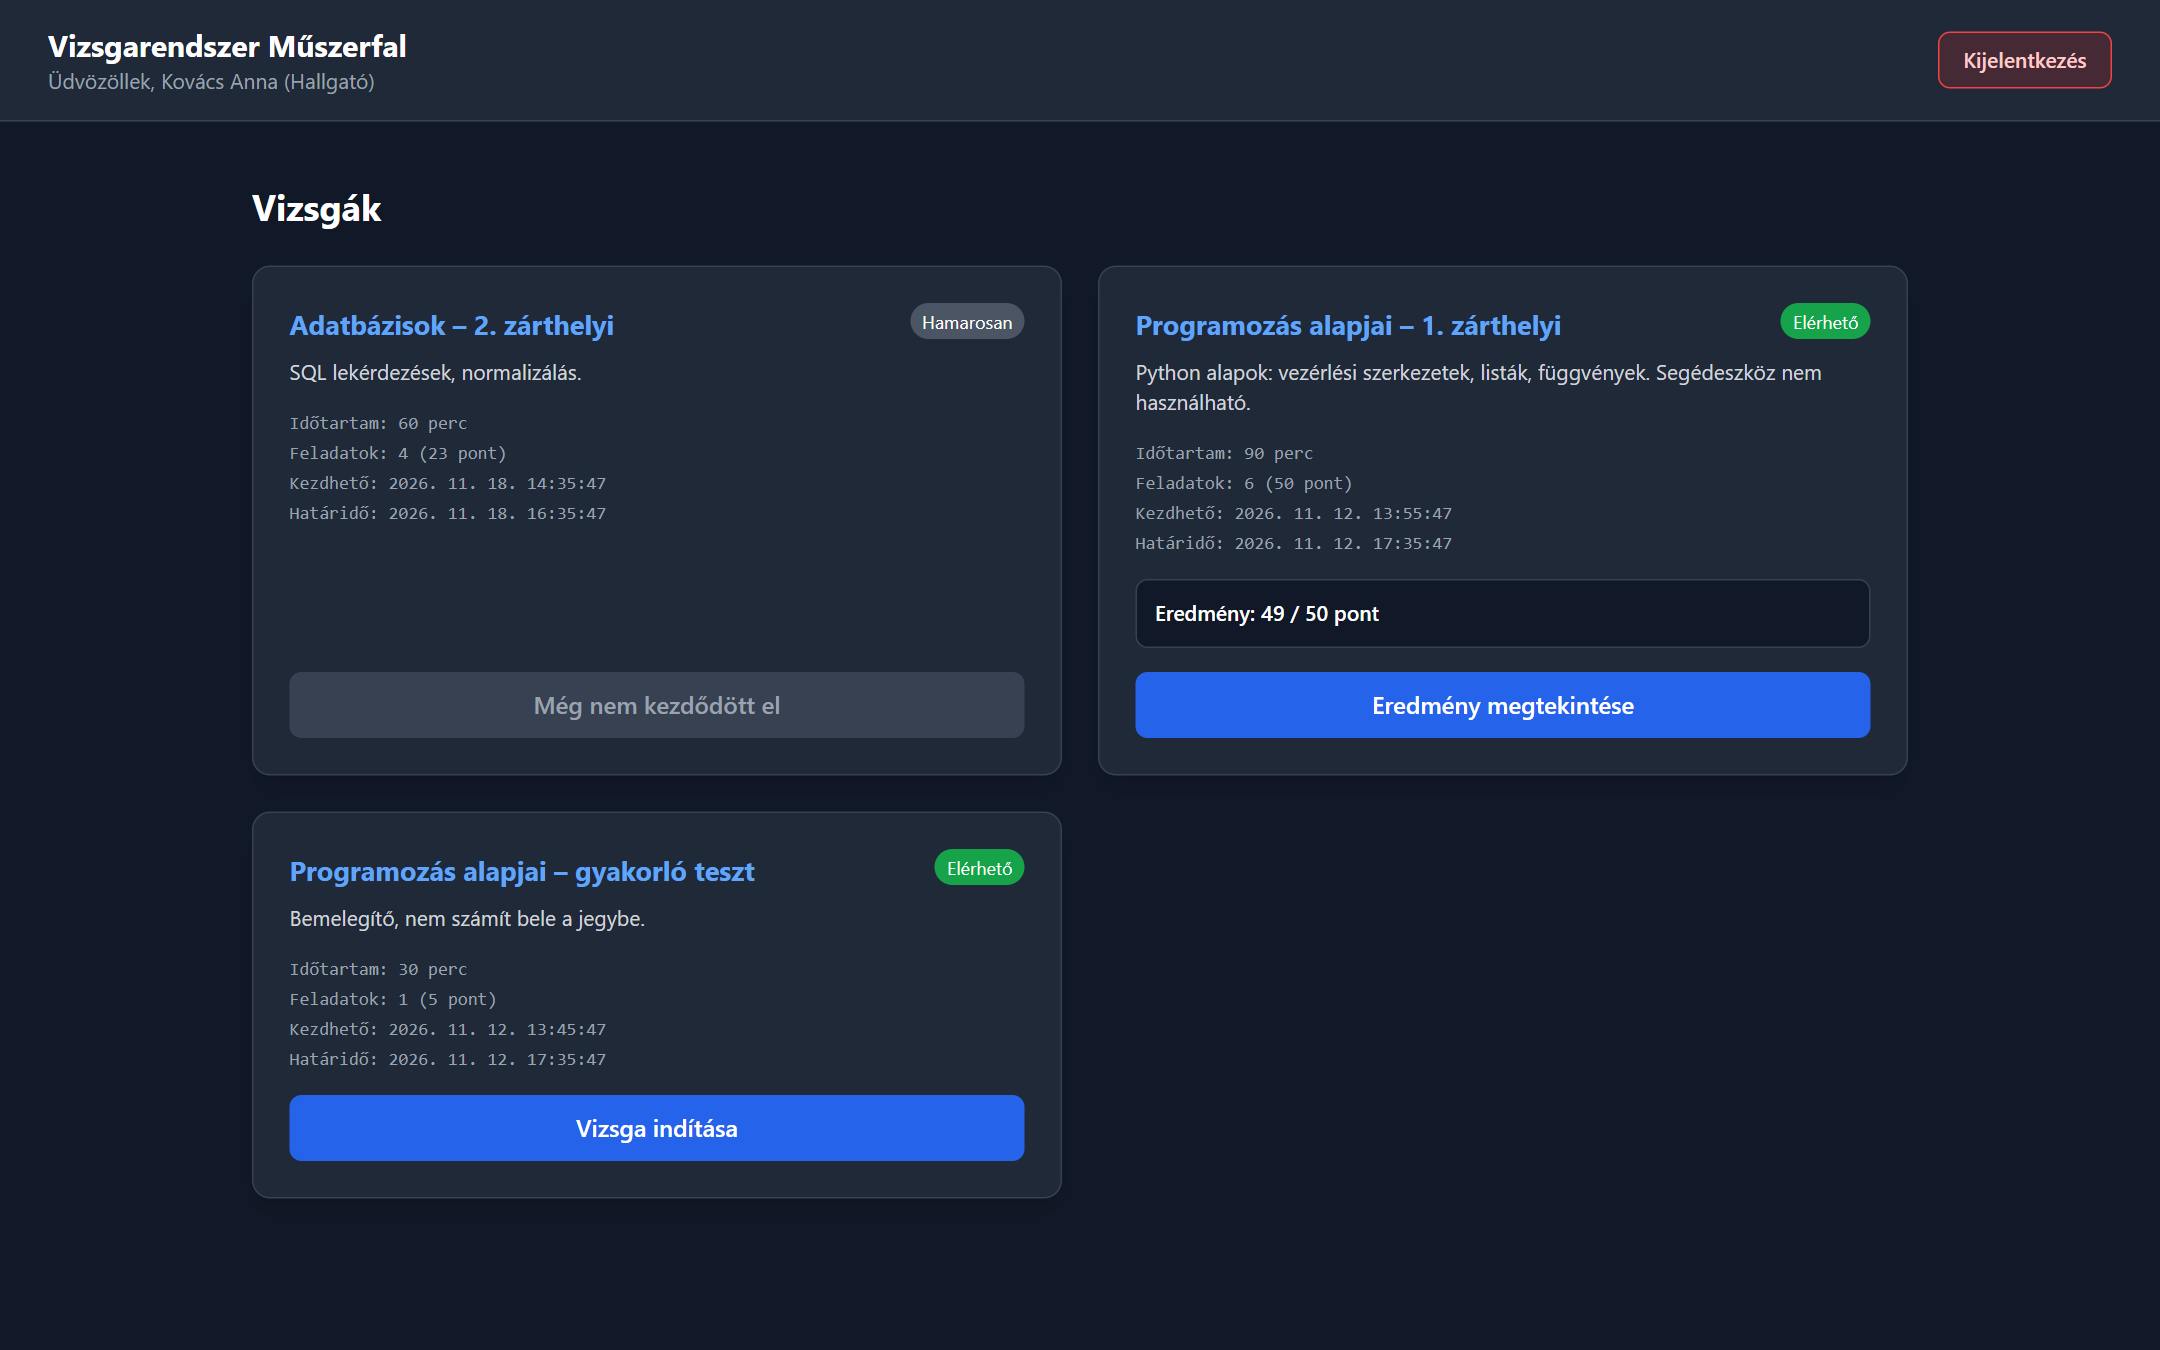
\includegraphics[width=\textwidth]{images/hallgatoi_muszerfal.png}
  \caption{A hallgatói műszerfal}
  \label{fig:hallgatoi_muszerfal}
\end{figure}

A vizsgaoldalt programozási feladattal \aref{fig:vizsgaoldal_kod}. ábra mutatta, választós
feladatnál a válaszlehetőségek jelölőnégyzetekként jelennek meg (\mref{fig:vizsgaoldal_valasztos}).
Több helyes válasz esetén a feladat szövege alatt figyelmeztetés jelzi, hogy a hibás jelölés
pontlevonással jár.

\begin{figure}[H]
  \centering
  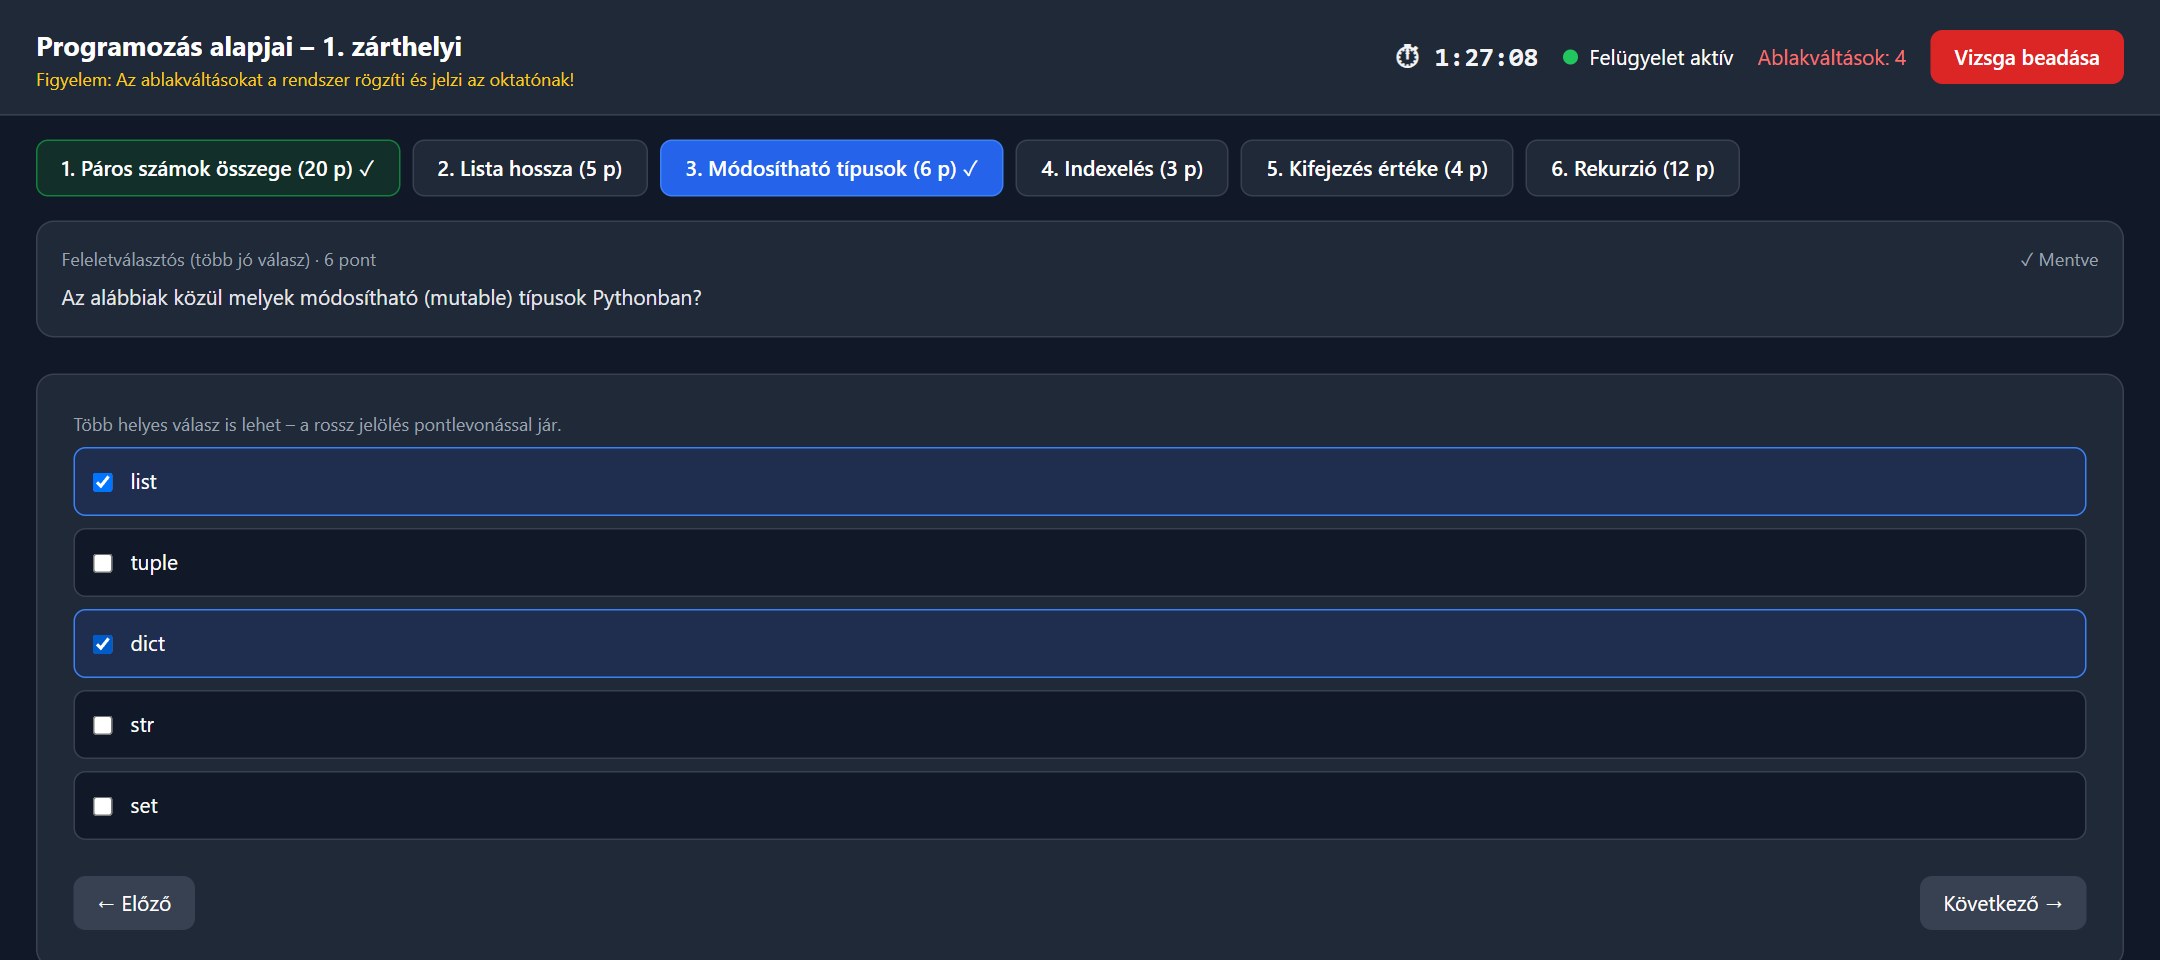
\includegraphics[width=\textwidth]{images/vizsgaoldal_valasztos.png}
  \caption{Több helyes választ tartalmazó feladat a hallgatói vizsgaoldalon}
  \label{fig:vizsgaoldal_valasztos}
\end{figure}

\section{Korlátok}
\label{sec:korlatok}

A tesztelés során a rendszer korlátai is világossá váltak. A kódfeladatok jelenleg csak Python
nyelven oldhatók meg, és az értékelés a kimenet szöveges egyezésén alapul, így a feladatkiírásnak
pontosan meg kell határoznia a kimenet formátumát. A böngészőalapú felügyelet egy második eszköz
használatát nem érzékeli, és egy hozzáértő hallgató a böngésző fejlesztői eszközeivel a jelzések
küldését is megakadályozhatja; a felügyelet tehát az oktató tájékoztatását szolgálja, nem
bizonyítékot szolgáltat. A kódértékelés szinkron módon fut, és a teljes futás idejére lefoglal egy
szálat a szerver szálkészletéből, ezért sok egyidejű beküldés esetén a szerver terhelhetősége
korlátozott lehet; ezt terheléses teszttel nem vizsgáltam. Ezek a korlátok egyben a továbbfejlesztés irányait is kijelölik, amelyekre az
összefoglalásban térek ki.

%!TEX root = ../dolgozat.tex
\chapter{Összefoglalás}
\label{ch:osszefoglalas}

Dolgozatomban egy olyan webes vizsgáztató rendszer prototípusát terveztem meg és készítettem el,
amely egy vizsgán belül vegyes feladattípusokat kezel, a programozási feladatokat elszigetelt
Docker-konténerben, tesztesetekkel automatikusan értékeli, és valós időben jelzi az oktatónak, ha
egy hallgató a vizsga közben elhagyja a vizsgaablakot.

A szakirodalom áttekintése során megismertem a számítógéppel támogatott értékelés lehetőségeit
és korlátait, a programozási feladatok automatikus értékelésének több évtizedes múltját, valamint
az online vizsgafelügyelet körüli szakmai és etikai vitát. A hasonló rendszerek vizsgálata azt
mutatta, hogy a vegyes feladattípusok, a biztonságos kódfuttatás és a valós idejű felügyelet
ritkán jelenik meg együtt, és ahol igen, ott jelentős üzemeltetési terhet jelent. Ezekre a
tapasztalatokra építve fogalmaztam meg a rendszer követelményeit.

A megvalósított rendszer hat feladattípust támogat. A zárt és a rövid szöveges feladatokat
automatikusan pontozza, a több helyes választ tartalmazó feladatoknál a hibás jelöléseket levonó
részpontozással, a rövid válaszoknál pedig a formai eltéréseket (kis- és nagybetűk, szóközök,
tizedesjel) figyelmen kívül hagyó összehasonlítással. A programozási feladatokat nyilvános és
rejtett tesztesetekkel értékeli, a kifejtős feladatokhoz pedig kézi javítási felületet és
visszajelzési lehetőséget biztosít. A vizsgafolyamatban a határidőt a szerver érvényesíti, a
válaszok automatikusan mentődnek, és a hallgató munkája akkor sem vész el, ha a vizsga közben
bezárja a böngészőt.

A tesztelés eredményei alapján a rendszer a kitűzött céloknak megfelel. A 32 funkcionális
teszteset mindegyike, valamint a valós idejű felügyelet 10 tesztesete is sikeres volt. A sandbox
biztonsági tesztjei igazolták, hogy a tervezett korlátozások a gyakorlatban is megállítják a
leggyakoribb támadásokat: a végtelen ciklust, a fork bombát, a túlzott memóriafoglalást, a hálózati
és a fájlrendszer-hozzáférést. Egy programozási feladat értékelése 20 teszteset esetén is
nagyjából egy másodperc alatt elkészül, ami annak köszönhető, hogy egy kiértékeléshez csak
egyetlen konténer indul. A felügyeleti jelzés helyi környezetben 10 milliszekundumon belül
eljutott az oktatóhoz.

Amit kevésbé sikerültnek tartok, az elsősorban a kódfuttatás eredményének feldolgozása: a
biztonsági tesztek során kiderült, hogy egy, az eredményjelölő szövegét kiíró program
megakaszthatta a saját értékelését. Bár ez a pontszám meghamisítására nem adott lehetőséget, és a
hibát véletlenszerű, futtatásonként generált jelölővel ki is javítottam, jól mutatja, hogy egy nem megbízható kódot futtató rendszernél a vezérlő és a
futtatott program közötti kommunikációt is ugyanolyan gondosan kell megtervezni, mint magát az
elszigetelést. Ez a tapasztalat egyben megerősítette bennem, hogy egy ilyen rendszernél a
szándékosan ártó bemenetekkel végzett tesztelés elengedhetetlen. A felügyelet terén pedig
tudatosan választottam a korlátozott, de a magánszférát tiszteletben tartó megoldást; véleményem
szerint egy egyetemi vizsgán ez jobb egyensúlyt jelent, mint a hallgatók kamerás megfigyelése,
ugyanakkor el kell fogadni, hogy egy elszánt hallgatót ez a módszer nem tart vissza.

A rendszer több irányban is továbbfejleszthető. A legkézenfekvőbb lépés további programozási
nyelvek (például C, C++ vagy Java) támogatása, amely a sandbox felépítésének köszönhetően
elsősorban a megfelelő konténerképek és a fordítási lépés hozzáadását jelentené. A kód
szerkesztését egy szintaxiskiemelést és automatikus kiegészítést nyújtó szerkesztő, például a
Monaco Editor beépítése tenné kényelmesebbé. Nagyobb létszámú vizsgák esetén a kódértékelést
egy üzenetsorra és külön feldolgozó folyamatokra (\textit{worker}) érdemes áthelyezni, hogy a
kiértékelés ne terhelje a webszervert, és a terhelés több gépre is szétosztható legyen. A
vizsgák tisztaságát a beküldött programok egymás közötti hasonlóságát vizsgáló plágiumkeresés
segíthetné, az oktatók munkáját pedig a feladatonkénti statisztikák (átlagpontszám, a sikertelen
tesztesetek eloszlása) és egy feladatbank, amelyből a feladatok több vizsgában is
újrahasznosíthatók. Végül egy LTI szabvány szerinti integráció lehetővé tenné, hogy a rendszer
egy meglévő tanulásirányítási rendszerbe, például a Moodle-be illeszkedjen, így a hallgatóknak nem
kellene külön fiókot létrehozniuk.

Összességében úgy érzem, hogy a dolgozat elkészítése során nemcsak egy működő rendszert hoztam
létre, hanem a webes alkalmazásfejlesztés, az informatikai biztonság és a konténerizáció terén
is olyan gyakorlati tapasztalatokat szereztem, amelyeket a későbbi szakmai munkám során is
hasznosítani tudok.


%biblatex verzió
%a bibintoc heading stílussal megjelenik a tartalomjegyzékben, title-lel a megjelenő címsor szövege módosítható
\printbibliography[heading=bibintoc,%
title=Források]
%sima bibtex verzió
%\bibliographystyle{plain}
%\bibliography{dolgozat.bib}

%!TEX root = ../dolgozat.tex
\pagestyle{empty}

\section*{Adathordozó használati útmutató}

A szakdolgozathoz mellékelt adathordozó a következő könyvtárakat és fájlokat tartalmazza:
\begin{itemize}
\item \texttt{dolgozat.pdf} -- a szakdolgozat PDF formátumban,
\item \texttt{dolgozat/} -- a szakdolgozat \LaTeX{} forráskódja,
\item \texttt{online-exam-system/backend/} -- a FastAPI alapú szerveroldali alkalmazás,
\item \texttt{online-exam-system/frontend/} -- a Next.js alapú kliensoldali alkalmazás,
\item \texttt{online-exam-system/docker-compose.yml} -- a PostgreSQL adatbázis indítását leíró fájl,
\item \texttt{online-exam-system/README.md} -- részletes telepítési és használati leírás,
\item \texttt{tesztek/} -- a \mref{ch:teszteles}ben ismertetett tesztszkriptek.
\end{itemize}

\subsection*{Futtatás}

A futtatáshoz Docker Desktop, Python 3.10 vagy újabb, valamint Node.js 18 vagy újabb verzió
szükséges. Az alkalmazás három lépésben indítható el, az \texttt{online-exam-system} könyvtárból:
\begin{enumerate}
\item Az adatbázis és a sandbox image előkészítése:\
  \texttt{docker compose up -d}\
  \texttt{docker pull python:3.11-slim}
\item A szerver indítása a \texttt{backend} könyvtárban:\
  \texttt{python -m venv venv}, majd a környezet aktiválása után\
  \texttt{pip install -r requirements.txt}\
  \texttt{uvicorn main:app --port 8000}
\item A kliens indítása a \texttt{frontend} könyvtárban:\
  \texttt{npm install}\
  \texttt{npm run dev}
\end{enumerate}
Ezután az alkalmazás a \texttt{http://localhost:3000} címen érhető el, az API interaktív
dokumentációja pedig a \texttt{http://localhost:8000/docs} címen. Oktatói fiók a regisztrációs
űrlapon az ,,Oktatóként regisztrálok'' lehetőséggel és az alapértelmezett \texttt{oktato123}
meghívókóddal hozható létre (ez a \texttt{TEACHER\_INVITE\_CODE} környezeti változóval
módosítható).

A tesztszkriptek a \texttt{backend} könyvtár virtuális környezetének Python értelmezőjével
futtathatók; paraméterként a \texttt{backend} könyvtár elérési útját kell megadni. A sandbox
tesztjéhez futó Docker szükséges.


\end{document}
